\chapter[Classifying High-Redshift Galaxies Spectra]{Clustering galaxy spectra at $0.5<z<1$: an unsupervised approach}
\label{ch: paper2}
\defcitealias{Hossein12}{T12}
\defcitealias{Kinney96}{K96}
\defcitealias{Noll09}{N09}

%----------------------------------------------------------------------------------------
%----------------------------------------------------------------------------------------
%----------------------------------------------------------------------------------------
%Intro
%----------------------------------------------------------------------------------------
%----------------------------------------------------------------------------------------
%----------------------------------------------------------------------------------------
\section{Introduction}
\label{sec: intro_somz}
%General information about SEDs
Nearly all information we can obtain from a galaxy is encapsulated in the light it emits; every observable phenomenon in a galaxy leaves a footprint on its spectral energy distribution (SED).
We can determine some physical property of a galaxy by properly modeling various features observed in its SED, and the general shape of the SED can be used as an identifier of the morphological type.
Considering the main features of SEDs, galaxies can be categorized into two main groups: elliptical or spiral.
Each group has its own characteristic features and can in turn be divided into many sub-branches.

%%Creating templates and NIR_UV templates
Several attempts have been made to create a complete set of templates for categorizing the spectral type of galaxies using data from nearby galaxies~(e.g.~\citealt{Kinney93}, \citealt[][hereafter \citetalias{Kinney96}]{Kinney96}, \citealt{Bershady00}, \citealt{Mannucci01}). 
Based on their usage, these templates are restricted to certain wavelengths.
In near-infrared (NIR) to ultraviolet (UV) wavelengths (the region where energy output of stars peaks), the SED contains information about the main physical properties of galaxies, e.g., age, star formation rate (SFR), stellar mass, metallicity, and interstellar medium.


% categorizing galaxies based on their SED

Advances in techniques and detectors have resulted in more detailed observations of SEDs and also made classification of galaxies more complex.
Since no two galaxies, even with the same morphology, have exactly the same properties, classifying SEDs of galaxies using templates is very challenging.
To overcome this challenge, many fitting methods have been developed and used to find template matches for SEDs, with $\chi^2$ minimization being the most commonly used. 
Artificial neural networks, K-means clustering, and principal component analysis are some other methods used to cluster and classify spectral types of galaxies based on their SED \citep[e.g.][]{Allen13,Ordov14,Shi15}.

%ANNs
Artificial neural networks (ANNs), which are inspired by the way neurons in a human brain route and process data, are very powerful tools that are used in data processing and pattern recognition problems.
An ANN contains many interconnected units (nodes or neurons) which process data and work together to solve problems.
It uses a set of training methods to learn about nonlinear and complex relations between input and output data, and how to apply these relations to new sets of data~\citep[e.g.][]{Hossein14,Hossein16,Ellison16a, Ellison16b}.
Studies have shown that ANNs outperform chi-square minimizing techniques and can be used as an alternative choice for fitting data~\citep[e.g.][]{Marquez91}.
Specifically, ANNs perform faster in large databases~\citep[][]{Gulati97}.

%Training methods for networks
Neural networks can be trained using two methods: supervised and unsupervised.
In supervised method, a neural network would be trained using input data based on a desired outcome.
This method is very useful for classification of data with specific target values.
On the other hand, in unsupervised method there is no prediction of output.
This method classifies data based on their underlying structures and hidden patterns.
The unsupervised method is very helpful to obtain knowledge from the data, or when the underlying structure of data is not well established.

%SOM
A Kohonen self-organizing map (also called self-organizing map, or SOM) is an unsupervised neural network for mapping and visualizing a complex and nonlinear high dimension data introduced by~\citet{Kohonen82}.
It shows simple geometrical relationships in non-linear high dimensional data on a map \citep{Kohonen98}.
%SOM in Astronomy
The utilization of the SOM in astronomy dates back to the 1990s, with \citet[][]{Odewahn92}, \citet[][]{Hernandez94}, and \citet[][]{Murtagh95} among the first to use SOMs in their studies.
\citet{Geach12} used COSMOS data to demonstrate two of the main applications of SOMs: object classification and clustering, and photometric redshift estimation. The latter has been the subject of many other studies \citep[e.g.][]{Kind14a}.
From classifying quasars' spectra to star/galaxy classifications, from gamma-ray bursts clustering to classification of light curves, this method has proved to be useful in various fields of astronomy \citep[e.g.][]{Maehoenen95, Miller96, Andreon00, Balastegui01, Rajaniemi02, Brett04, Scaringi09}.


%SOM in Astronomy continued.
Large spectroscopic surveys have made available integrated spectra of millions of galaxies.
These integrated spectra combine the light of billions of individual stars and nebulae within a galaxy, and
finding patterns and common characteristics between galaxies can be a complex task.
\citet{In12} introduced a new clustering tool based on the SOM method for analyzing these large datasets.
They used $\sim 60000$ spectra from the Sloan Digital Sky Survey \citep[SDSS;][]{Abazajian09} to test their tool, and created very large SOMs to analyze the type of spectra/objects.
They also generated SOMs from quasars' spectra in order to find unusual types of spectra. 
Later, \citet{Meusinger16} used these SOMs and updated data from SDSS and other surveys to find a new class of quasars.
The other application of SOMs is to find outliers or errors in the data.
\citet{Fustes13} produced a package based on SOM to classify spectra from the GAIA survey that were previously classified as ``unknown'' by the SDSS pipeline. This package can recognize an astronomical object from instrumental errors, and then classify the object based on its spectrum.

%What \citetalias{Hossein12} did
~\citet[][hereafter \citetalias{Hossein12}]{Hossein12} classified spectral types of a sample of 142 galaxies using a supervised (Multi-layer feed-forward) neural network method, based on the spectral template presented by \citetalias{Kinney96}.
With the supervised method, they could only classify spectral types of 105 out of the 142 galaxies.
The spectra of the 37 galaxies from their samples could not be matched with any of those in the \citetalias{Kinney96} templates. 
In order to classify the remaining 37 galaxies, they combined spectrum of the \citetalias{Kinney96} templates.
\citetalias{Hossein12} also showed that there are tight correlations between physical properties of galaxies, and these correlations might be different for each type of galaxy.

%What we did
In this paper, we compare supervised and unsupervised methods of galaxy spectral classification directly, using exactly the same data as \citetalias{Hossein12}.  
Our hypothesis was that since a self-organizing map has the freedom to classify objects in between known classes, it could be applied to this data 
to find the best spectral class for the 37 galaxies that could not be classified by the supervised method.
First, we train self-organizing maps using the \citetalias{Kinney96} spectral templates and compare our classification with the \citetalias{Kinney96} classification.
Then, we use the trained network to classify the spectra of 142 galaxies with $0.5 < z < 1$ from \citetalias{Hossein12}. 
As in \citetalias{Hossein12}, we examine the averaged properties of the new galaxy groups and compare them with previous work.
In Section $\S$~\ref{sec: data_highZ}, we present the data that we use to train and test our networks. 
We describe the SOM methods in Section $\S$~\ref{sec: method_somz}. 
The results of the spectral classifications and a comparison with previous studies are presented in Section $\S$~\ref{sec: result}. 
In Section $\S$~\ref{sec: summary_SOMZ}, we summarize our results and discuss potential future work in this subject.
%----------------------------------------------------------------------------------------
%----------------------------------------------------------------------------------------
%----------------------------------------------------------------------------------------
%DATA
%----------------------------------------------------------------------------------------
%----------------------------------------------------------------------------------------
%----------------------------------------------------------------------------------------

\section{Data}
\label{sec: data_highZ}
We use spectra templates from \citetalias{Kinney96} to train neural networks.
To test the trained networks, we use SED and physical properties of 142 galaxies at $0.5<z<1$ from \citetalias{Hossein12}.
Following the \citetalias{Hossein12} work, we chose these two sets of data not only to show the application of SOMs in spectra clustering, but also to easily compare supervised and unsupervised methods.

 \subsection{Kinney Spectral Model}
     \begin{figure}
        \centering
        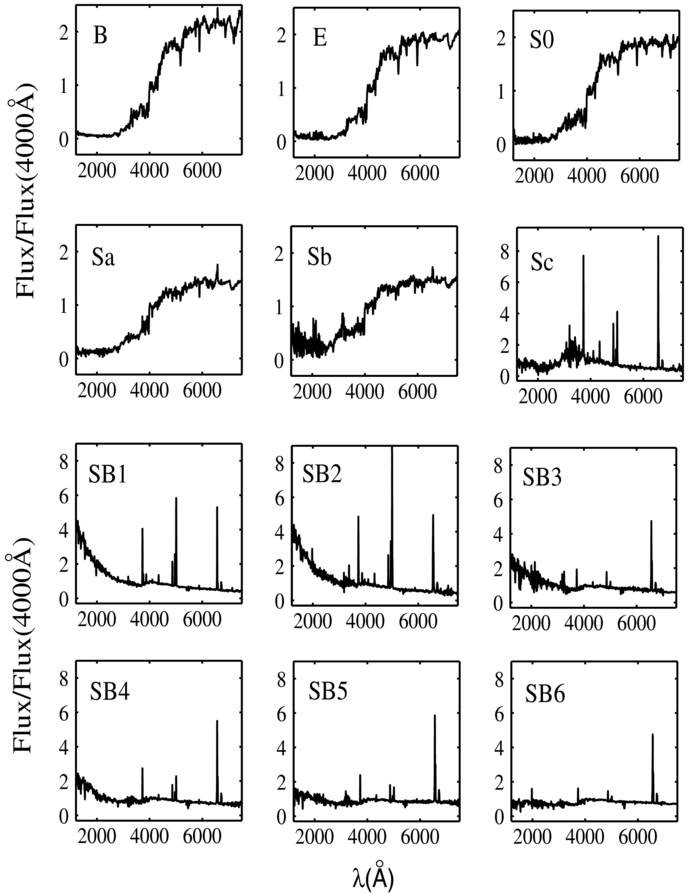
\includegraphics[width=0.9\textwidth]{../image_paper2/k96.jpg}
        \caption[\citet{Kinney96} spectra template for 12 types of galaxies]{\citet{Kinney96} spectra template for 12 types of galaxies from \citet{Hossein12} paper (Fig. 1 in \citet{Hossein12}). The type of each template is shown in each frame. Plots B, E, S0, Sa, Sb and SC show spectra that belong to the quiescent galaxies. Starburst galaxies spectra are indicated with SB 1 to 6. Higher numbers represent more intrinsic colour extinction.}
        \label{fig: k96}
    \end{figure}
      
    \citetalias{Kinney96} used ultraviolet-optical spectra of 70 star forming and quiescent nearby galaxies to produce a set of templates that contained 12 types of spectra templates.
    These templates have been widely used in many studies to determine morphological type of galaxies or properties of specific types of galaxies~\citep[e.g.][]{Shakouri16, Paiano16, Laporte16, Holden16}.
    \citetalias{Kinney96} stated that these templates can also be used to classify the spectra of high-redshift galaxies. 
    
    The 12 templates are divided based on their morphological types for quiescent galaxies or their extinction for starburst galaxies (Fig.~\ref{fig: k96}). 
    The quiescent group of galaxies includes Bulge (B), Elliptical (E), S0, Sa, Sb, and Sc galaxies.
    The bulge group represents galaxies similar to M31 and M81, whose UV and optical spectra are dominated by their bulge stellar populations.
    The starburst galaxies are divided into six groups (SB1 to SB6) based on their intrinsic extinctions ($E(B-V)$). 
    As Fig.~\ref{fig: k96} shows, SB1 galaxies have lower internal extinctions ($E(B-V) \simeq 0.05$), while SB6 galaxies have the highest amount of extinction ($E(B-V) \simeq 0.65$) among starburst galaxies. 
    In the quiescent (B to Sb) templates, the spectrum is redder; strong absorption lines and the 4000~\AA~break are distinguishable.
    SEDs of starburst galaxies are flatter in the optical and near-infrared region than those of the quiescent ones and show strong emission lines.
    For more details on each spectral type, we encourage readers to see \citetalias{Kinney96} and references therein. 
   The \citetalias{Kinney96} spectra span from $\sim1200$~\AA~to $10000$~\AA~with a resolution of $\sim 10$~\AA.
    However, in this work we only use $\sim1200< \lambda < 8000$~\AA~to train our networks; 
    this wavelength range was chosen due to availability of flux information in those wavelengths for all 12 templates. 

 \subsection{SED and Properties of the Sample Galaxies} 
    \citetalias{Hossein12} selected 142 galaxies from the spectroscopic campaign of the ESO GOODS-South field~\citep{Vanzella05, Vanzella06, Vanzella08}.
    The 142 galaxies were selected based on the availability of photometry from HST/ACS, VLA/ISAAC, and {\it Spitzer}/MIPS and IRAC (10--13 filters with $\sim 0.4<\lambda<24~\mu$m in the observed frame).
   Data from these instruments was necessary in order to have a complete picture of stellar population and star formation rate. 
    For each galaxy, a robust spectroscopic redshift and photometric measurements from the GOODS-MUSIC catalogue \citep{Santini09} was available.
   \citetalias{Hossein12} matched the point spread function (PSF) of the photometric data with \citetalias{Kinney96} data and used the photometry as inputs to the Code Investigating GALaxy Emission ({\em CIGALE});~\citep[][hereafter N09]{Noll09} to generate the best-fit SED for each galaxy.
    \citetalias{Hossein12} produced the best SED match, with wavelength interval of 910~\AA~to $\sim 80$~cm, for each galaxy\footnote{This wavelength interval is the default output of the {\em CIGALE} code}.
    Assuming decreasing SFR and visual attenuation ($\tau$) model, Salpeter initial mass function~\citep{Salpeter55}, and old stellar population with age of $\sim 10$~Gyr, they derived physical properties of the galaxies such as age and stellar mass.
    Some of these properties are shown in Table~\ref{tab: props}.
    In Section~\ref{sec: 1D_somz}, we study these properties for each category.
    More details on creating SEDs and extracting information about galaxy properties using {\em CIGALE} can be found in \citetalias{Noll09} and \citetalias{Hossein12}.
    
       
\begin{table}
\caption[Description of the properties of \citet{Hossein12} galaxies]{Description of the properties of \citet{Hossein12} galaxies; the output result of {\em CIGALE}}     
\label{tab: props}
\centering
\begin{tabular}{l l l}
\hline\hline
\noalign{\smallskip}
Par. & Unit & Description\\
\noalign{\smallskip}
\hline
\noalign{\smallskip}
$t_{\,\mathrm{oSP}}$ & Gyr & age of old SP model \\
$t_{\,\mathrm{ySP}}$ & Gyr & age of young SP model \\
$f_\mathrm{burst}$ & --- & mass fraction of \\
& & young single population (SP) model \\
\noalign{\smallskip}
$t_{\,\mathrm{D4000}}$ & Gyr & D4000-related age \\
\noalign{\smallskip}
$M_\mathrm{star}$ & M$_\odot$ & total stellar mass  \\
SFR & M$_\odot$/yr & instantaneous SFR  \\
$A_\mathrm{FUV}$ & mag & attenuation at 1500\,\AA{} \\
\noalign{\smallskip}
\hline
\end{tabular}
\end{table}

    For testing the created networks, we use SEDs that were produced by \citetalias{Hossein12}. 
    These SEDs are publicly available~\footnote{All the \citetalias{Hossein12} produced SEDs can be found in \href{http://telbib.eso.org/detail.php?bibcode=2012AJ....144..172T}{ESO webpage}} in the form of flux per rest frame wavelength in a wide range of wavelengths.
    Since we have used the \citetalias{Hossein12} SEDs to test the trained network, we only used the part of the SEDs that have the same wavelength range as the \citetalias{Kinney96} spectral templates.  

%----------------------------------------------------------------------------------------
%----------------------------------------------------------------------------------------
%----------------------------------------------------------------------------------------
%Method
%----------------------------------------------------------------------------------------
%----------------------------------------------------------------------------------------
%----------------------------------------------------------------------------------------
\section{Method}
\label{sec: method_somz}
 \subsection{Self Organizing Maps}
 \label{sec: som_SOMZ}
  The SOM is a clustering method which reduces the dimensionality of data, while preserving topological features~\citep{Kohonen98}. 
 The results of the SOM are shown with a map of neurons, which their numbers are set by the user.
 Each neuron has a fixed position in the map and may contain one or more samples from the input data in a n-dimensional space,~\boldit{V} $\in \Re^n$.
 A weight vector,~\boldit{W} $\in \Re^n$, with the same dimension as the input data, is associated with each node and will be varied during the training process.
 The process of creating an SOM happens over a series of $N$ iterations.
 In each iteration, the algorithm calculates the Euclidean distance for each node $j$ as $D_j^2= \sum_{i=0}^{i=n} (V_i - W_i)^2$, and finds a neuron with $D_{j_,\mathrm{min}}$. 
 This neuron is the winner node and is calling Best Matching Unit (BMU). 
 In each iteration (t), the weight vectors W(t) in the neighbourhood of the BMU ($r^t_{BMU}$) will change according to the Kohonen learning rule (equation~\ref{equ: weight adj}). 
  \begin{equation}
            \label{equ: weight adj}
            W(t+1)=W(t)+L(t) \times R(t) \times(V(t)-W(t))
 \end{equation}
where $L(t) = L_0 e^{(-t/\tau)}$ is the learning factor with $L_0$ is the initial value of learning, which prevents the divergence of the SOM, and $R(t)=\exp(-\frac{D_j^2}{2r^t_{BMU}})$ is the influence rate, which determines how the weight of each node will change. 
$\tau$ is the number of total iterations.
Values for the number of neurons is arbitrary, and for various toolboxes values for one or all of $L_0$,$L(t)$, $R(t)$  and $r^t_{BMU}$ are arbitrary.
\cite{Geach12} demonstrate the algorithm of the SOM in more detail.


     The same as Chapter~\ref{ch: paper3}, we use the \textsc{matlab} neural network toolbox~\citep[NNT,][]{matlabtolbox} to create self-organizing maps.
     To present our results in this chapter, we use {\sc nnt}'s built-in plotting tool.
     Specifically, we use two of the plots in this tool: a hits map, which shows the number of times each neuron has became the winner (hits), and a distance map, which shows the distance between those neurons.
     In the maps, the purple hexagonal shapes represent the neurons. 
     The distances in a distance map are shown by the grey cycle colours:
     the darker the colour, the larger the distance between neurons.
     In the hit maps, neurons with zero hits are left empty.

       
    The sizes of the SOM maps are arbitrary and there are no rules regarding choosing one over the other. 
    \citet{Vesanto05} suggested that a total number of $5\sqrt{n}$ neurons is a sufficient size, but users usually choose the size of the grids based on their dataset and their application of the results.

   
% \subsection{Mock Sample}
 
%          \begin{figure}
%             \begin{subfigure}[b]{0.5\textwidth}
%                 \centering
%                 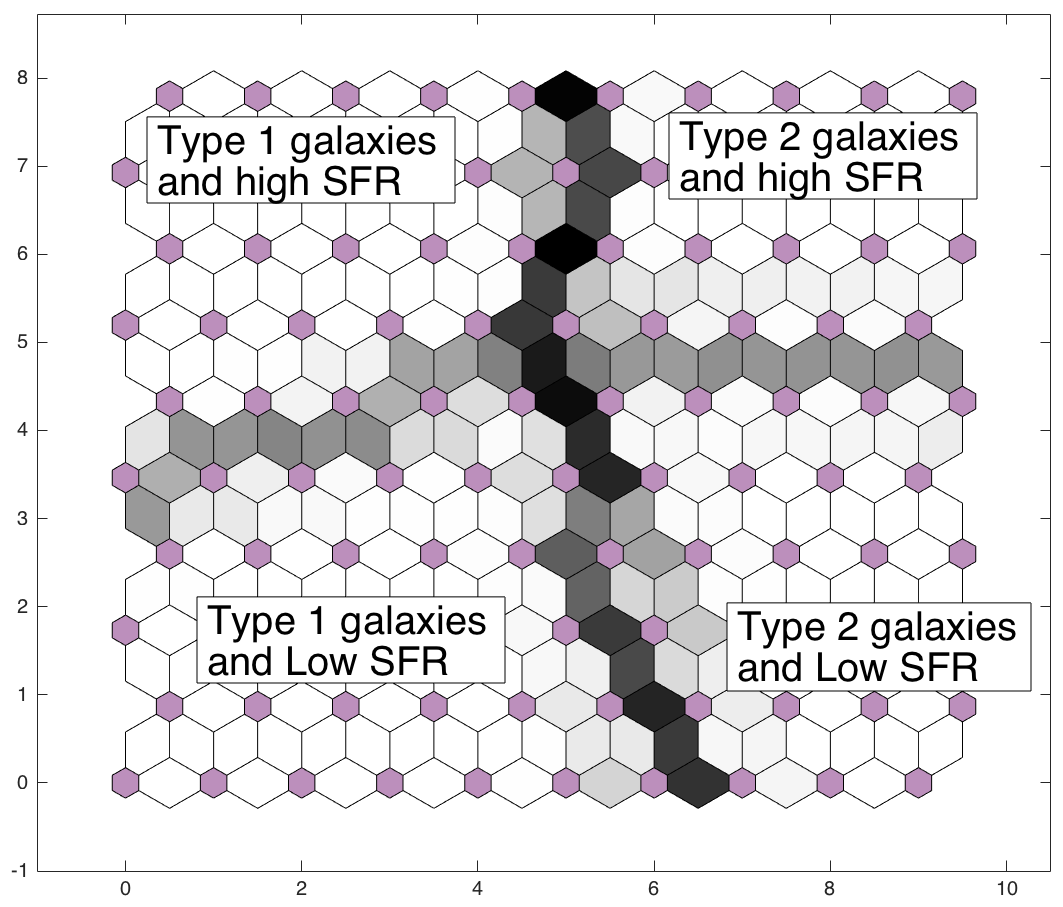
\includegraphics[width=\textwidth]{../image_paper2/sample/sample2_dist.png}
%             \end{subfigure}
%             \hfill
%             \begin{subfigure}[b]{0.5\textwidth}
%                 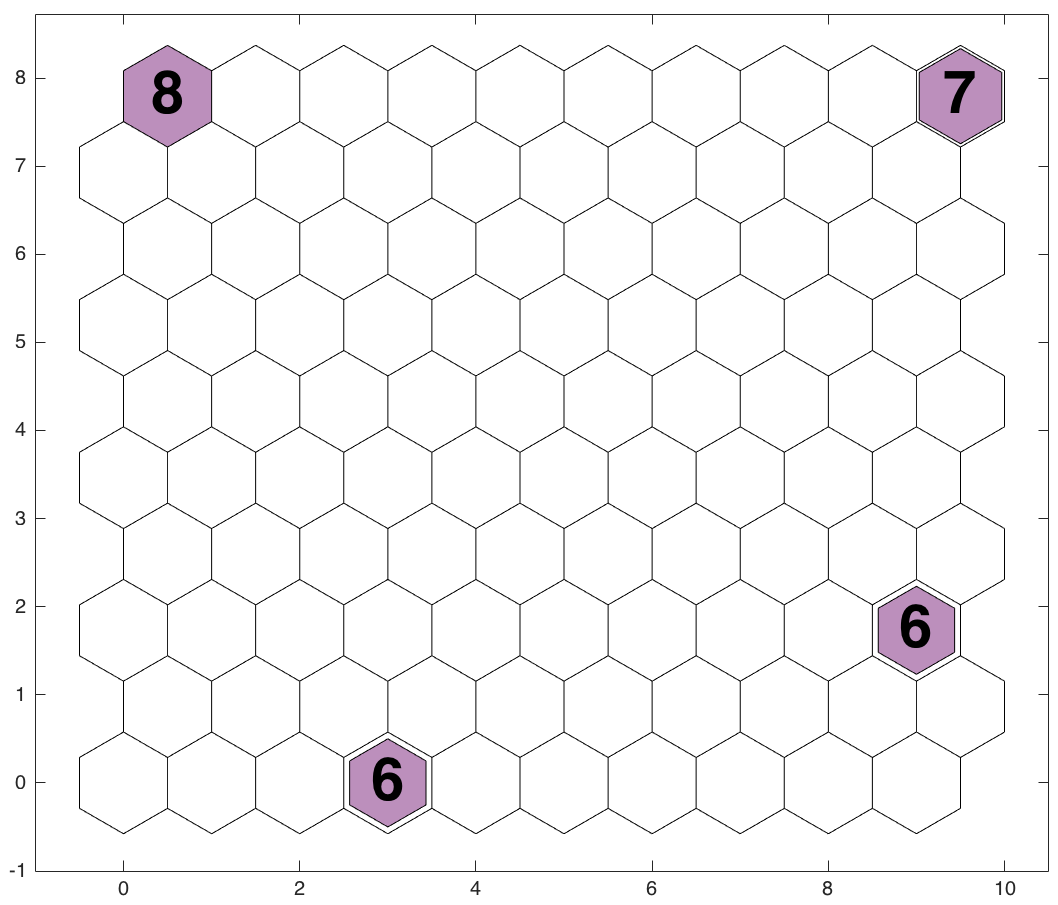
\includegraphics[width=\textwidth]{../image_paper2/sample/sample2_hits.png}
%             \end{subfigure}
%             \caption[Self-organizing map of the mock sample]{SOM of the mock sample. In both plots, the axes show the position of the neurons. Hexagonal shapes represent the neurons. The top plot is a distance map. The grey cycle colours show the differences between the weights of each neuron with white being the minimum difference and black being the maximum one. The lower plot is a ``hits plot". It represents the number of samples in each neuron, where empty means zero hits. In this sample, the 27 galaxies are clustered in 4 groups, containing 8, 7, 6 and 6 galaxies respectively.}
%             \label{fig: sample}
%         \end{figure}
 
%  To illustrate how self-organizing maps work, we create a mock sample of 27 galaxies.
%  The mock sample contains two attributes for each galaxy: the type (type 1 or type 2), and the star formation rate (high or low). 
%  We generated a SOM of size $10 \times 10$ using the same initial values mentioned in Section~\ref{sec: create_som}.

%  Fig. ~\ref{fig: sample} shows the SOM of this mock sample. 
%  The upper panel is the distance map. 
%  The axes show the position of the neurons in the $10 \times 10$ network.
%  The lower panel in Fig.~\ref{fig: sample} shows the hit map.
%  On this map, similar to the distance map, the axes show the position of the neurons and the hexagonal shapes are the neurons.
%  The number on the purple neurons shows the number of galaxies in that neuron.
%  Colour coverage of neurons depends on the number of the hits on the sample.
%  The neuron with the maximum number of hits is dark-coloured while the empty neurons are left uncoloured (white).
 
% Using this method, as expected, we are able to divide the mock sample galaxies into 4 distinct groups: Type 1 with high SFR, type 1 with low SFR, type 2 with high SFR and type 2 with low SFR. 
% The upper panel in the Fig.~\ref{fig: sample} clearly shows this division.
% In that plot, the upper half belongs to high star forming galaxies, while the lower half belongs to low star forming galaxies.
% The left half of the plot is where type 1 galaxies belong, and type 2 galaxies reside in the right side.
% Different shades of gray show the border between regions.
% The lower panel in Fig.~\ref{fig: sample} shows that only 4 neurons (out of 100) are occupied. 
% 8 galaxies are type 1 galaxies with high SFR, 7 are type 2 galaxies with high SFR, 6 are type 1 galaxies with low SFR and the other 6 are type 2 galaxies with low SFR. 
% We can conclude that although each galaxy had  the chance to occupy any of the neurons in the network, because of the similarity in the values of their attributes, they remained only in four groups.
% This network is considered a training network and can be used to cluster any new dataset with similar entries.


% As we show in the following sections, with data from real galaxies there are more than two dimensions and two galaxies never have exactly the same information. 
% If the network has enough neurons, the input data points would eventually separate from each other and cluster into smaller groups. 
% However, if the input data has high similarity, the number of neurons must be much higher than the number of input samples to be able to separate the groups from each other. 
% Therefore, it is up to the users to decide the similarity or dissimilarity between the input data based on number of neurons. 

%----------------------------------------------------------------------------------------
%----------------------------------------------------------------------------------------
%----------------------------------------------------------------------------------------
%Results
%----------------------------------------------------------------------------------------
%----------------------------------------------------------------------------------------
%----------------------------------------------------------------------------------------
%\include{sections_highz/}{results.tex}
%----------------------------------------------------------------------------------------
%----------------------------------------------------------------------------------------
%----------------------------------------------------------------------------------------
%Results
%----------------------------------------------------------------------------------------
%----------------------------------------------------------------------------------------
%----------------------------------------------------------------------------------------
\section{Results and Discussion}
\label{sec: result}

    In this section we show the results of the neural networks trained using the \citetalias{Kinney96} template spectra.
    Training with \citetalias{Kinney96} templates results in networks that have regions corresponding to galaxies of known morphological type. 
    The trained networks can then be used to categorize other galaxies.

    In order to find a sufficient size for the trained networks, we created maps with sizes ranging from $1\times2$ to $50\times50$.
    Varying the grid size of the maps helps us to monitor whether tighter grouping of galaxies is due to their similar properties or a lack of map space to separate them.
   Based on the size of the data and SOM results, we found the optimum grid size to be $1\times22$ and $12\times12$ in 1D and 2D maps, respectively. 
    For each grid we created different SOMs with different learning factors, neighbourhood distances, and number of iterations to find the optimum.
    We create the final SOMs with initial values for number of iterations in ordering phase, ordering phase learning factor, tuning phase learning factor, and tuning phase neighbourhood distance of 1000, 0.9, 0.02, and 1, respectively.
   
    We started our analysis by creating 1D SOMs. 
    First, we created SOMs with only two neurons ($1\times2$ map), and then increased the number of neurons one at a time in the 1D case (Section~\ref{sec: 1D_somz}).
    We generate 2D networks (Section~\ref{sec: 2D}),  again starting with the smallest possible number of neurons (4 neurons in a $2\times2$ map), increasing to 144 in a $12\times12$ map.    
    For each generated network, we compare the results with the \citetalias{Kinney96} categorization.
    We also use these networks to classify the \citetalias{Hossein12} galaxy sample, and compare this classification with that from the supervised networks in \citetalias{Hossein12}.

    \subsection{One-Dimensional Self-Organizing Maps}
    \label{sec: 1D_somz}
        \subsubsection{Training the Networks}
        \label{sec: 1Dt}
            To start our clustering, we assumed that galaxies can be divided into only two general types; quiescent and starburst.
            This corresponds to a network with only two neurons.
            We increased the size of the map gradually until the 12 input samples divide into the 12 neurons. 
        
            Figs.~\ref{fig: 1by2T} --\ref{fig: 1by22T} show the results of the training networks.
            As in to Fig.~\ref{fig: sample}, the upper part of the figures shows the neurons and their relative distances between weight of neurons.
            As mentioned in Section~\ref{sec: method_somz}, an increase in the darkness of colours between neurons represents an increase in relative distance between the neurons.
            The lower panels of the figures show the number of \citetalias{Kinney96} templates that are placed in each neuron. 
            \begin{figure}
                \begin{subfigure}[b]{\textwidth}
                    \centering
                  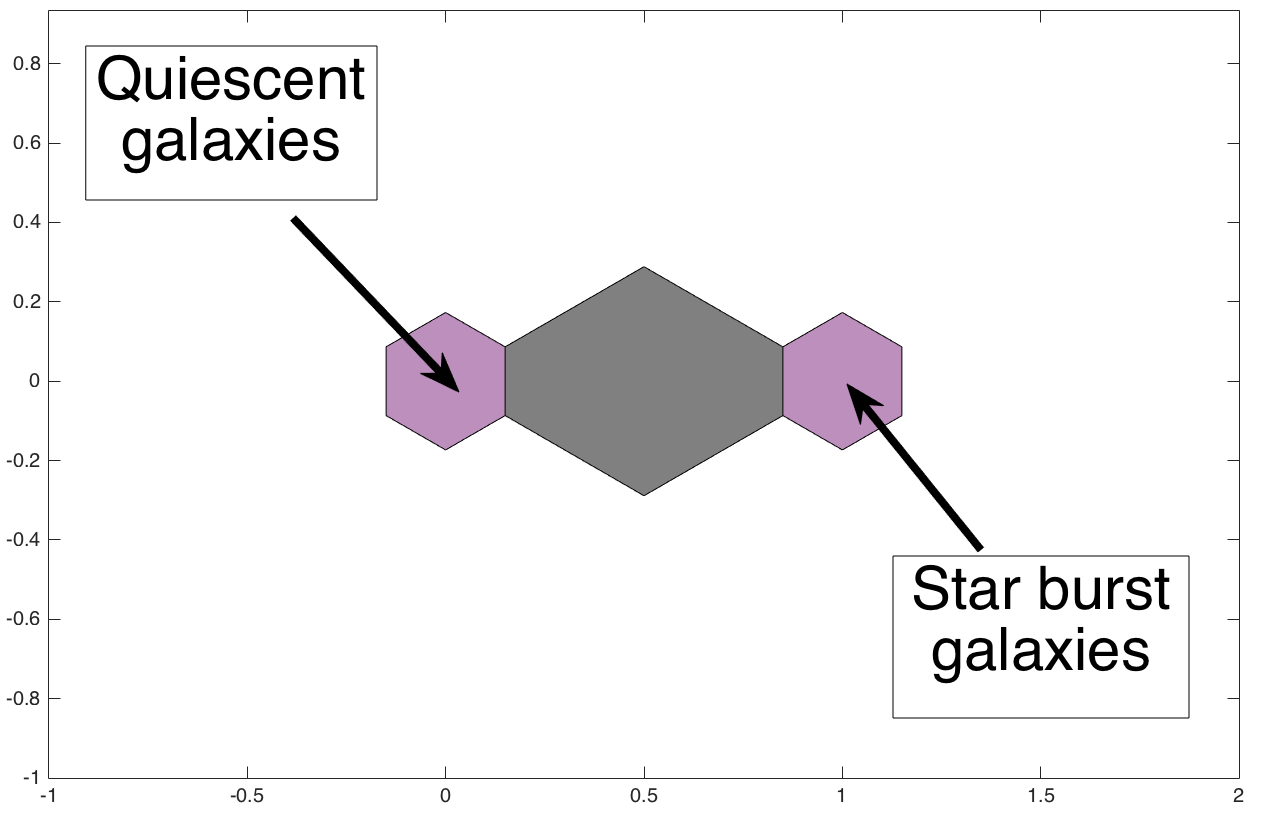
\includegraphics[width=0.8\textwidth]{../image_paper2/1d/dist_1_by_2.png}
                \end{subfigure}
                \hfill
                \begin{subfigure}[b]{\textwidth}
                    \centering 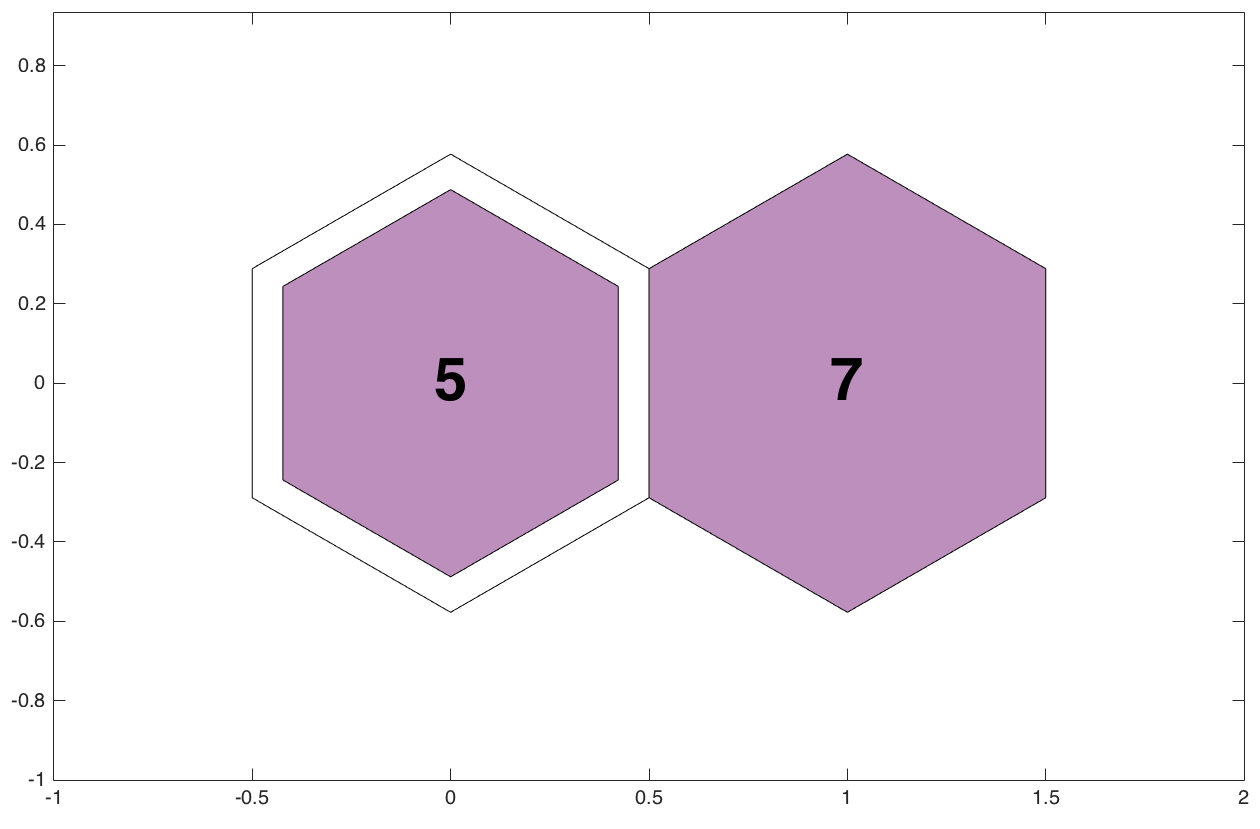
\includegraphics[width=0.8\textwidth]{../image_paper2/1d/hit_t_1_by_2.png}
                \end{subfigure}
                \caption[Results of training network in $1\times2$~grid]{Results of training network in $1\times2$~grid. As in Fig.~\ref{fig: sample}, the upper panel is a distance map and the lower panel is a hit map. In this network, 5 of the templates from \citet{Kinney96} are categorized as quiescent galaxies and the rest are starbursts. Because of their strong emission lines, Sc galaxies are moved towards the starburst ones.}
                 \label{fig: 1by2T}
            \end{figure}
        
        
            In the upper map in Fig.~\ref{fig: 1by2T}, the dark colour between two neurons indicates that the relative distance between these two groups are relatively high, and these two groups are distinguishable groups.
            In the lower part of Fig.~\ref{fig: 1by2T}, we see that the templates are divided into two groups of 5 and 7.
            Although we know from \citetalias{Kinney96} and \citetalias{Hossein12} that 6 of the templates are quiescent and the other 6 are starbursts, the SOM results show 5 of the galaxies in one group and the other 7 in the second group.
            In this method, the Sc template has been categorized as starburst due to the relatively higher disk stellar population relative to that of the bulge. 
            According to \citetalias{Kinney96}, Sc galaxies are considered to be late Hubble type galaxies which have a flattter spectra compare to other quiescent galaxies. 
            

            Fig.~\ref{fig: 1by3T} shows the results of the training in a 1$\times$3 network.
            In these plots we force the galaxies to be categorized in a maximum 3 groups. 
            If the templates in Fig.~\ref{fig: 1by2T} truly belonged in two groups, they would be grouped into two groups in this network, even when we try to cluster them into three. 
            However, in the lower panel of Fig.~\ref{fig: 1by3T}, we can see that the middle node contains two templates.
            These two templates, which are separated from the group of starburst templates in the lower part of Fig.~\ref{fig: 1by2T},  are the SB5 and SB6 types.
            In the upper plot of Fig.~\ref{fig: 1by3T}, the colour between two right neurons is black and the colour between two left neurons is white. 
            The black colour indicates that the left neuron is completely different from the other two groups,
            while the white colour shows that the two right neurons are very similar to one another. 
            
            Comparing Fig.~\ref{fig: 1by2T} to Fig.~\ref{fig: 1by3T} shows that the starburst templates are divided into two groups. 
            Based on the colours between these two groups, we conclude that they are very similar; both groups are starbursting and have strong emission lines.
            On the other hand, the SB5 and SB6 templates have the highest internal extinctions; this causes the spectra to become flatter at shorter wavelengths. 
            The flatter UV spectra makes these two templates more similar to quiescent galaxies than to other starbursts.
            Therefore, in the networks, SB5 and SB6 types are to be grouped close to the quiescent galaxy templates.
                
            \begin{figure}
                \begin{subfigure}[b]{\textwidth}
                    \centering
                    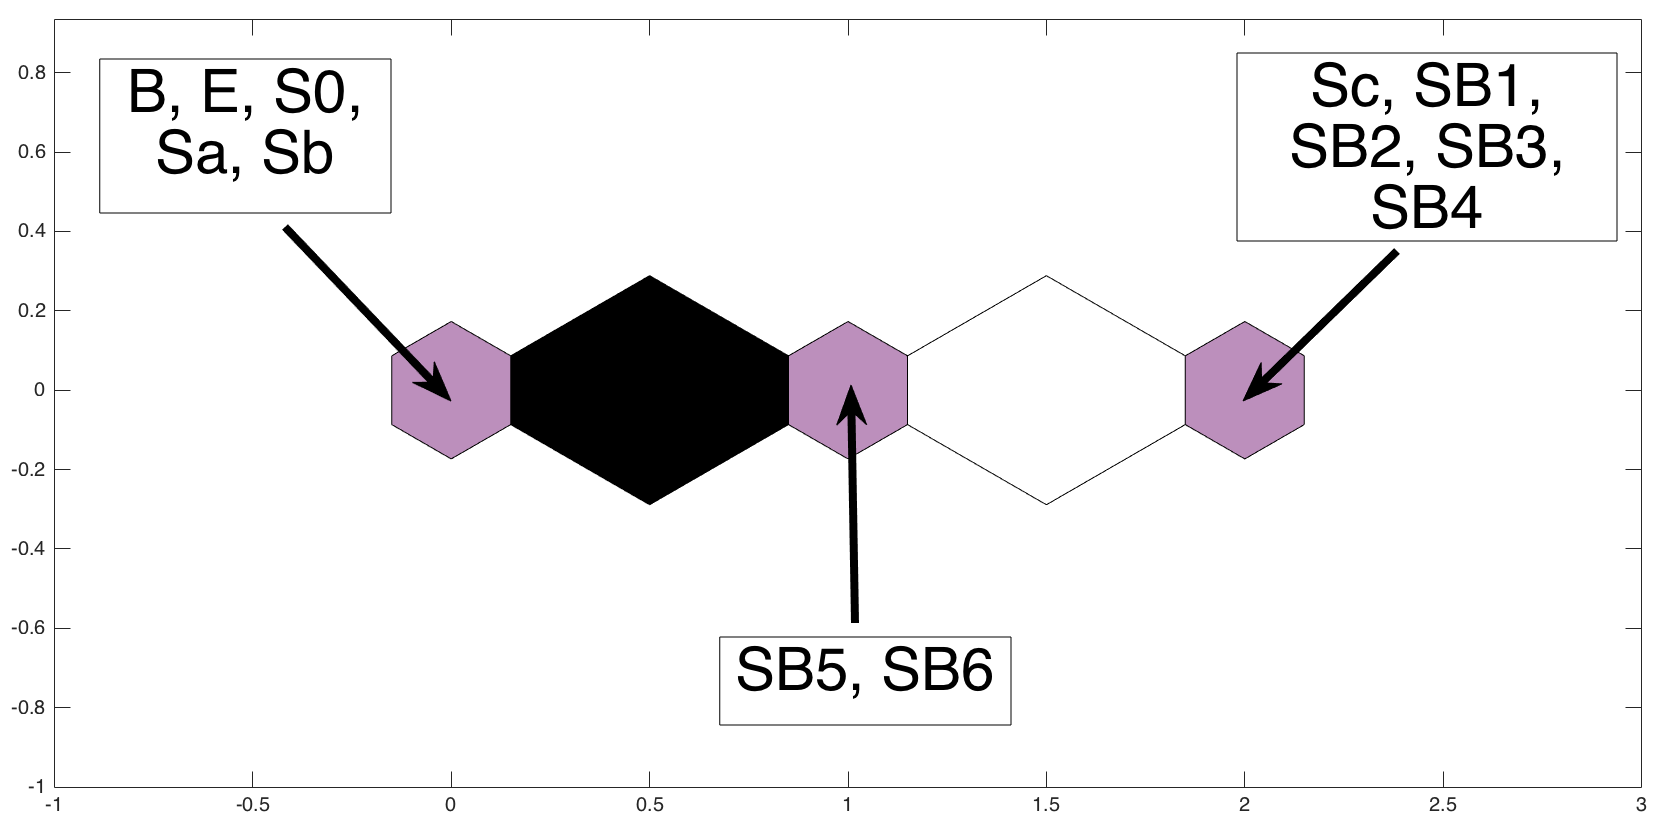
\includegraphics[width=\textwidth]{../image_paper2/1d/dist_1_by_3.png}
                \end{subfigure}
                \hfill
                \begin{subfigure}[b]{\textwidth}
                     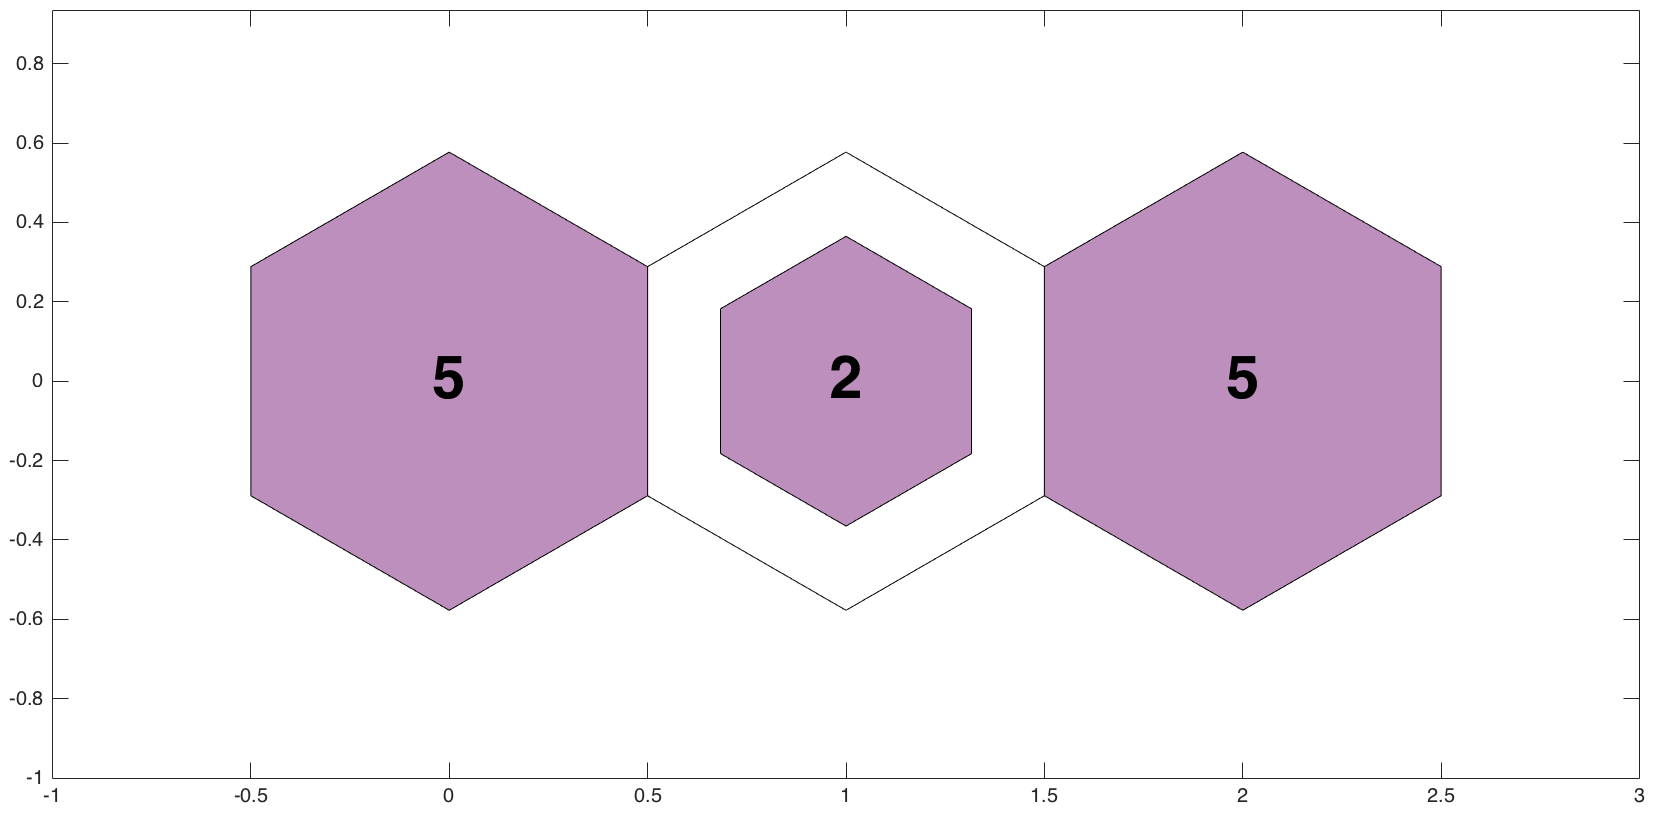
\includegraphics[width=\textwidth]{../image_paper2/1d/hit_t_1_by_3.png}
                \end{subfigure}
                \caption[Results of training network in $1\times3$~grid]{The same as Fig.~\ref{fig: 1by2T} but showing the results of training network in $1\times3$~grid. In this network again, 5 of the \citet{Kinney96} templates are categorized as quiescent and 7 as starbursts. However, this time 2 templates (SB5 and SB6) are separated from the starburst groups.}
                 \label{fig: 1by3T}
            \end{figure}
           
            We increased the size of the maps gradually until the galaxies are divided into twelve groups (Figs.~\ref{fig: 1by4T} to ~\ref{fig: 1by20T} in Appendix~\ref{app: high_Z_1d_soms} and ~\ref{fig: 1by22T}).
            Since there are more nodes in higher grid SOMs, the algorithm 
            pays more attention to small differences between groups.
            If the templates from \citetalias{Kinney96} had completely distinct spectral types, then a $1\times12$-sized SOM would be expected to show 12 different groups each containing a single template.
            However, in Fig.~\ref{fig: 1by12T}, we see that three of the neurons contain two templates and three of them are empty.
            It is evident that there was no template in the \citetalias{Kinney96} sample that can fill those empty neurons.
            In Fig.~\ref{fig: 1by12T}, from left to right, templates with types B and E, SB3 and SB4, and SB1 and SB2 are the ones grouped together. 
            The SB3 and SB4 grouping breaks when we increase the size of the network to $1\times15$~(Fig.~\ref{fig: 1by15T}).
            The SB1 and SB2 templates, however, remain in the same neuron until the size of the map is increased to $1\times20$~(Fig.~\ref{fig: 1by20T}).
            The separation between templates B and E only happens when the size of the SOM exceeds $1\times22$~(Fig.~\ref{fig: 1by22T}).
        \begin{figure}
            \begin{subfigure}[b]{\textwidth}
                \centering
                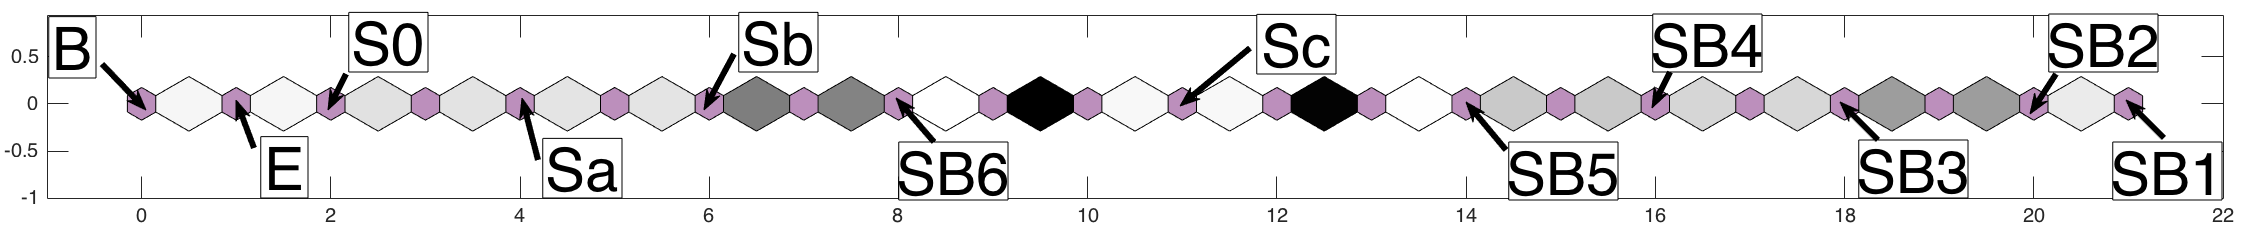
\includegraphics[width=\textwidth]{../image_paper2/1d/dist_1_by_22.png}
            \end{subfigure}
            \hfill
            \begin{subfigure}[b]{\textwidth}
                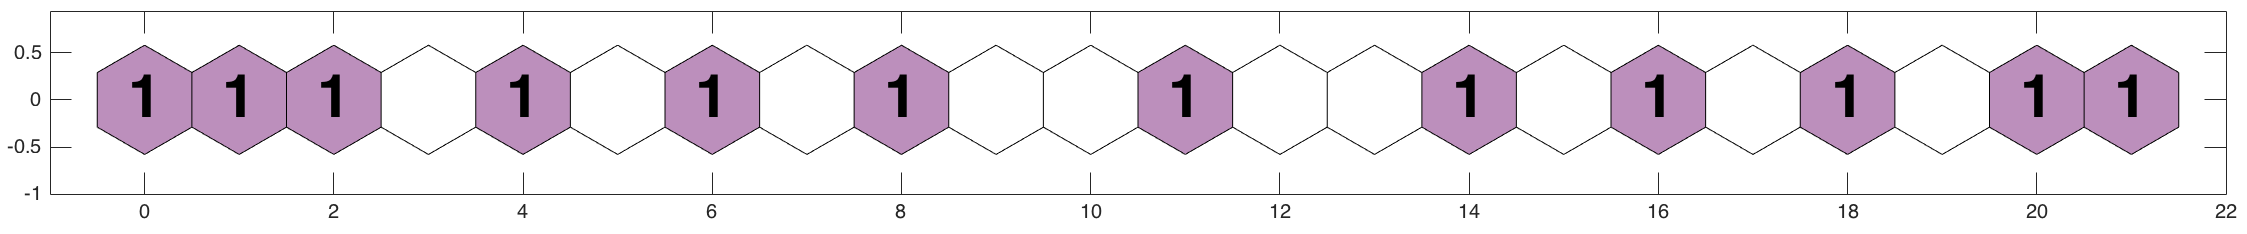
\includegraphics[width=\textwidth]{../image_paper2/1d/hit_t_1_by_22.png}
            \end{subfigure}
            \caption[Results of training network in $1\times22$~grid]{The same as Fig.~\ref{fig: 1by2T} but this time the figure shows results of training network in $1\times22$~grid.}
            \label{fig: 1by22T}
        \end{figure} 
    
            In Fig.~\ref{fig: 1by22T}, we can see twelve different groups:
            5 groups in the left-side neurons are separated from 7 groups on the right side of the map with two dark-grey colours between them.
            This shows that even though the galaxies are clustered in twelve groups, there still remain only two main distinct groups.
            The closest occupied neuron in the starburst side of the SOM, belongs to the SB6 type. 
            This template has the most extinction and its spectra has more similarity to quiescent galaxies than other starburst types. 
            
            The fact that the templates need to have at least 22 different neurons to be divided into 12 groups shows that the differences between SB1 and SB2, and B and E, templates are very small.
            Because of their similarities, they tend to stay in the same group until the network becomes big enough to make attention to the smallest particularity.
           
        \subsubsection{Classifying the Galaxy Sample}
         \label{sec: 1Dv}
            After training the networks as discussed in Section~\ref{sec: 1Dt}, we used them to classify the fitted SEDs of the sample of 142 galaxies from \citetalias{Hossein12}.
            The upper panel in Fig.~\ref{fig: 1by2V} shows the result of this classification using the $1\times2$~network from Fig.~\ref{fig: 1by2T}.
            Eighty of the galaxies have spectral types similar to those of the quiescent galaxies and the spectral types of the rest are similar to the starburst galaxies.
            The lower left panel shows the median spectra of the 80 galaxies that were classified as quiescent. 
            These galaxies are similar to the ones in the left node in the upper panel of Fig.~\ref{fig: 1by2T}:
            the spectra clearly show the 4000\AA~break, one of the signatures of quiescent galaxies.
            The H$\alpha$ emission in the spectrum could be from galaxies with similar spectral types to Sa galaxies, but with stronger emission lines.
            The median spectra in the lower right panel of Fig.~\ref{fig: 1by2V} shows strong emission lines and bright ultraviolet continuum, indications of a high star formation rate.
            \begin{figure}
                \begin{subfigure}[b]{\textwidth}
                    \centering
                    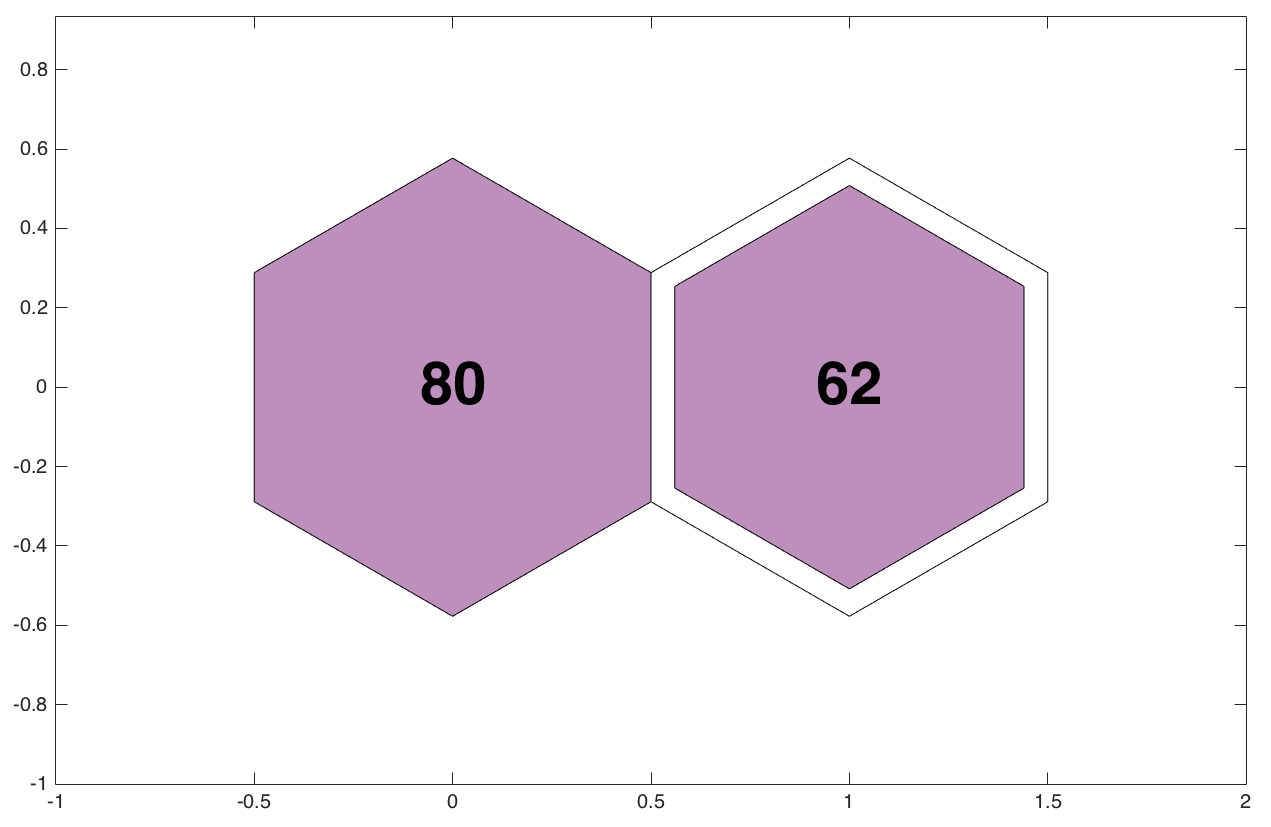
\includegraphics[width=\textwidth]{../image_paper2/1d/hit_v_1_by_2.png}
                    %\caption{$1\times2$ weight map}
                     %\label{fig: 1by3T}
                \end{subfigure}
                \hfill
                \begin{subfigure}[b]{\textwidth}
                     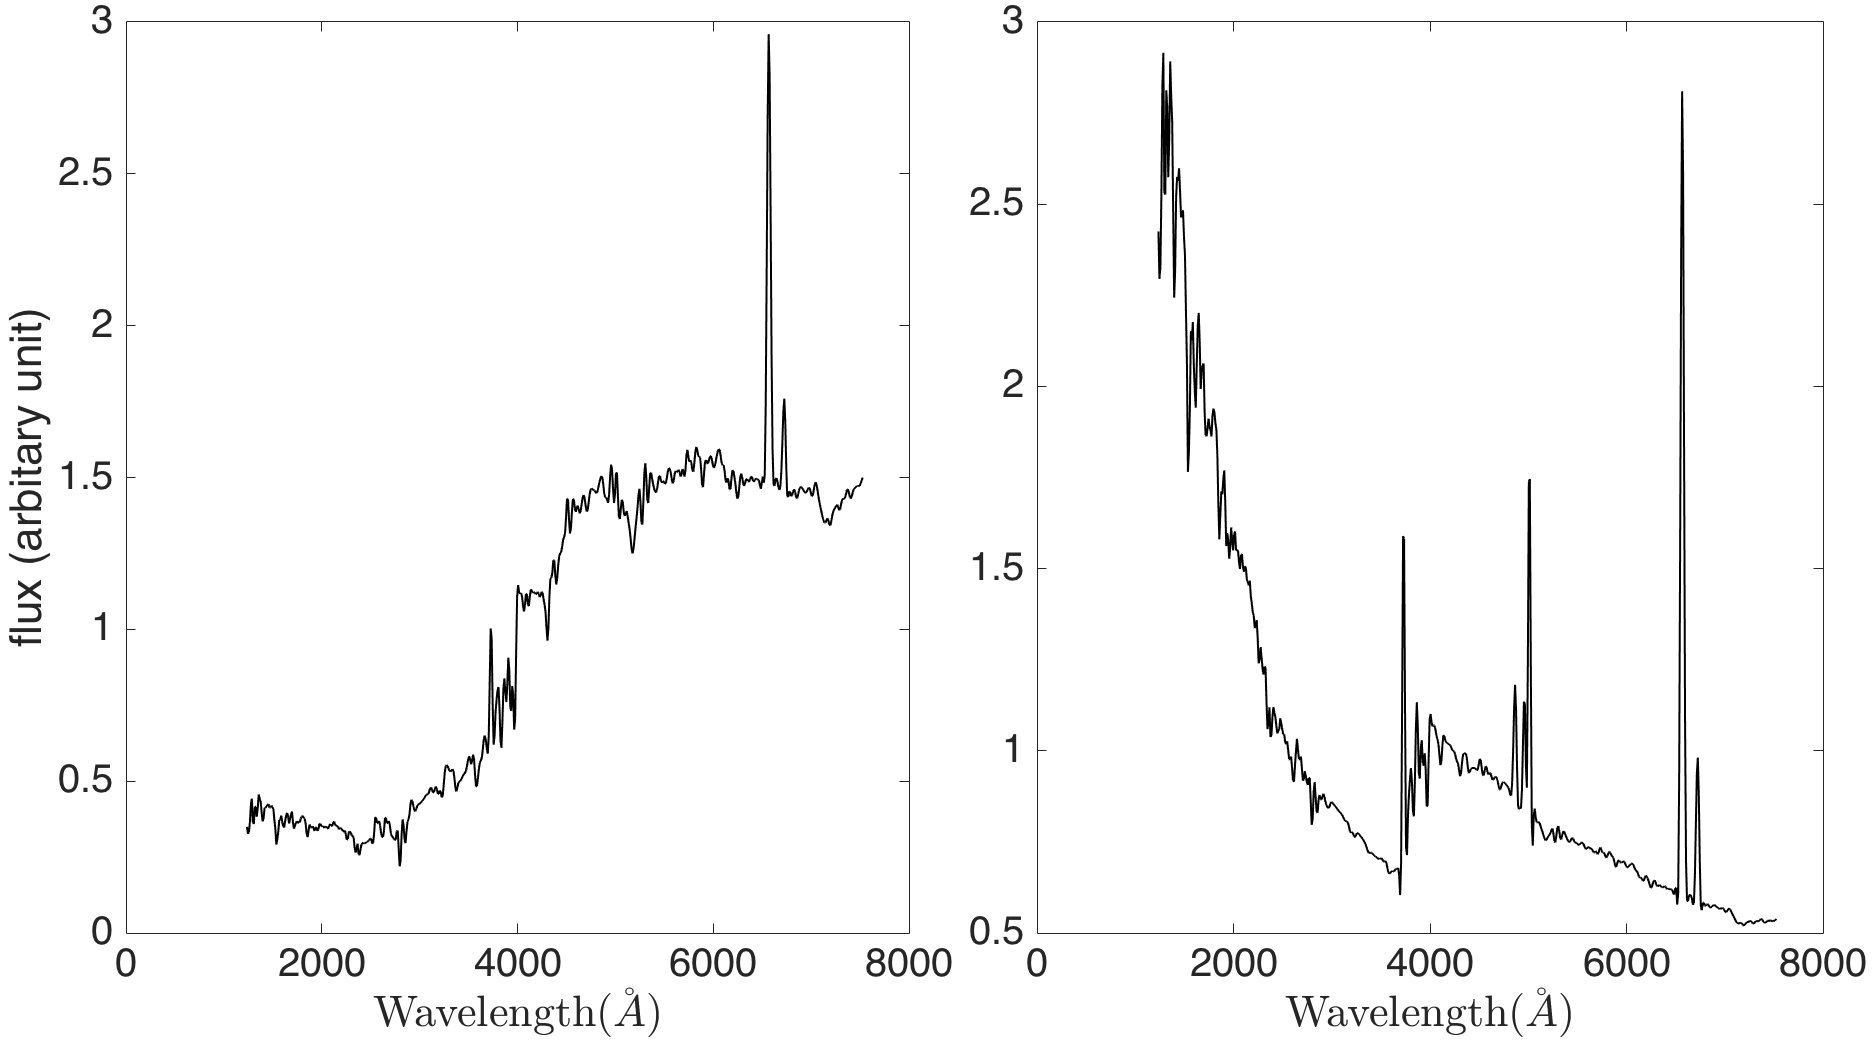
\includegraphics[width=\textwidth]{../image_paper2/1d/SED_total1by2.png}
                     %\caption{$1\times2$ hits map}
                     %\label{fig: 1by3Thits}
                \end{subfigure}
                \caption[Classification of fitted galaxy SEDs from \citet{Hossein12} using the $1\times2$~networks]{Classification of fitted galaxy SEDs from \citet{Hossein12} using the $1\times2$~network trained from the \citet{Kinney96} templates (Fig.~\ref{fig: 1by2T}). Upper panel: a hit map with the number in each node representing the number of galaxies belonging to that group. In this case 80 means that 80 of the 142 spectra are classified into the quiescent group while the 62 of the 142 spectra are categorized as starburst galaxies. Lower panel: median spectra of the galaxies in each group (fluxes are normalized by dividing spectra by flux at 4000\AA), early-type on the left and starburst on the right.}
                \label{fig: 1by2V}
            \end{figure}          
            
            Since in this network galaxies were forced to be divided into a maximum of two groups, the strongest feature in a galaxy's spectra predominantly decides which group the galaxy belongs to.
            Galaxies with a weak 4000\AA~break but strong emission lines and ultraviolet upturn are categorized as starbursts while galaxies with a strong 4000\AA~break are categorized as quiescent.
            Increasing the size of the SOM helps solve the problem of the galaxies which have features that are common in both groups.
            
            Fig.~\ref{fig: 1by3V} presents the result of classifying the spectra of the galaxies using the $1\times3$~network (from Fig.~\ref{fig: 1by2T}): 66 of the galaxies belong to the quiescent group, and 47 belong to the starburst group. 
            However, 29 of the galaxies are similar to starbursts in some, but not all, of their features. 
            Galaxies in this group have strong emission lines and are ultraviolet-bright, but they also have a strong 4000\AA~break, which makes them cluster closer to the quiescent galaxies (middle panel in the lower part of Fig.~\ref{fig: 1by2V}).

            \begin{figure}
                \begin{subfigure}[b]{\textwidth}
                    \centering
                    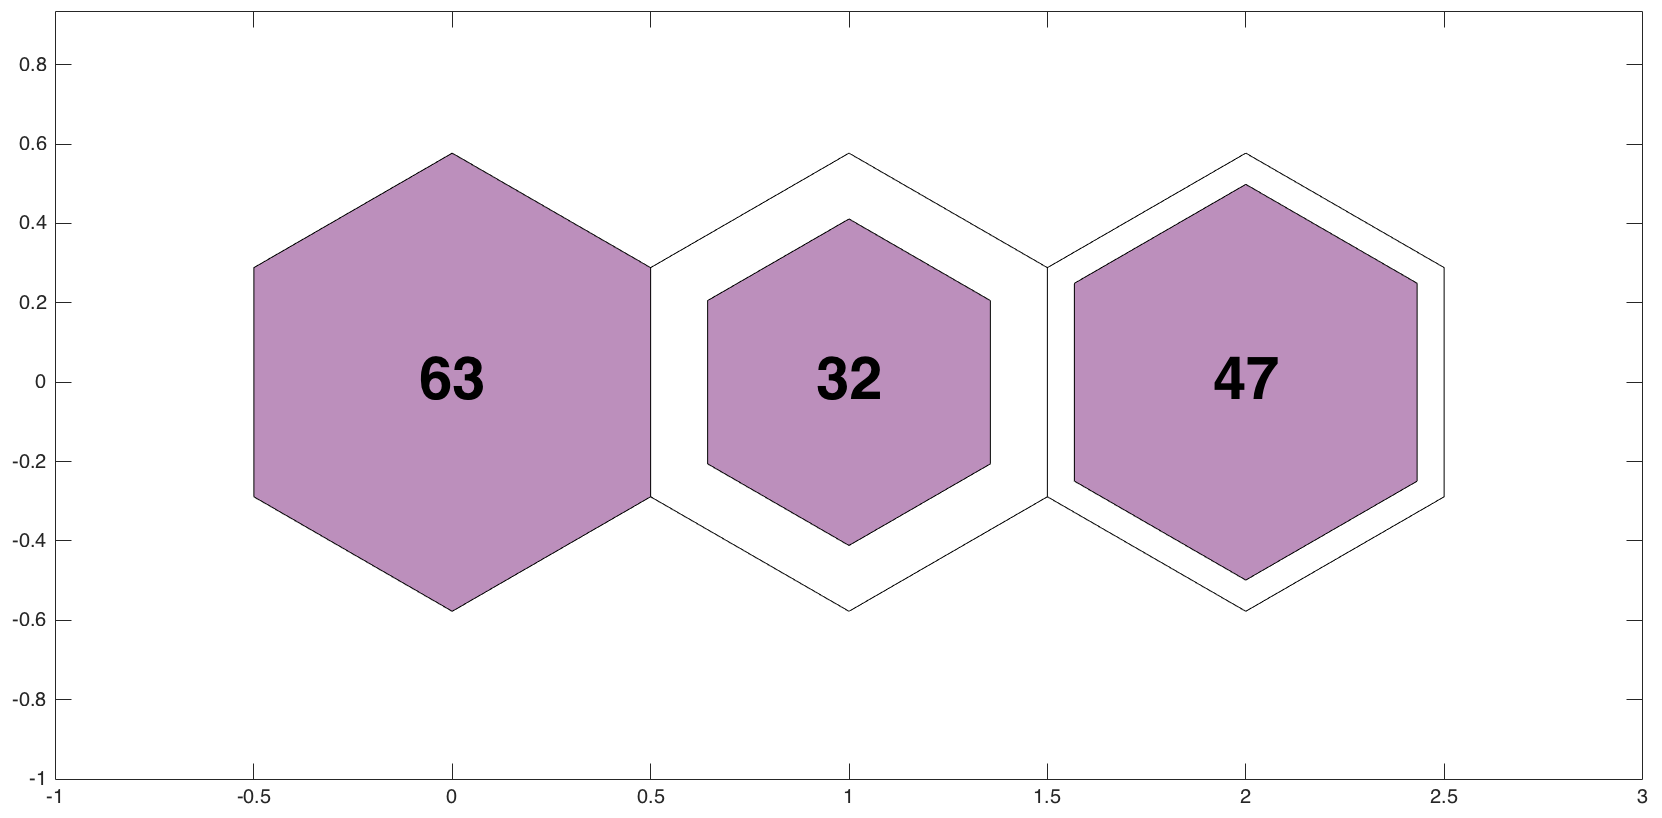
\includegraphics[width=\textwidth]{../image_paper2/1d/hit_v_1_by_3.png}
                \end{subfigure}
                \hfill
                \begin{subfigure}[b]{\textwidth}
                     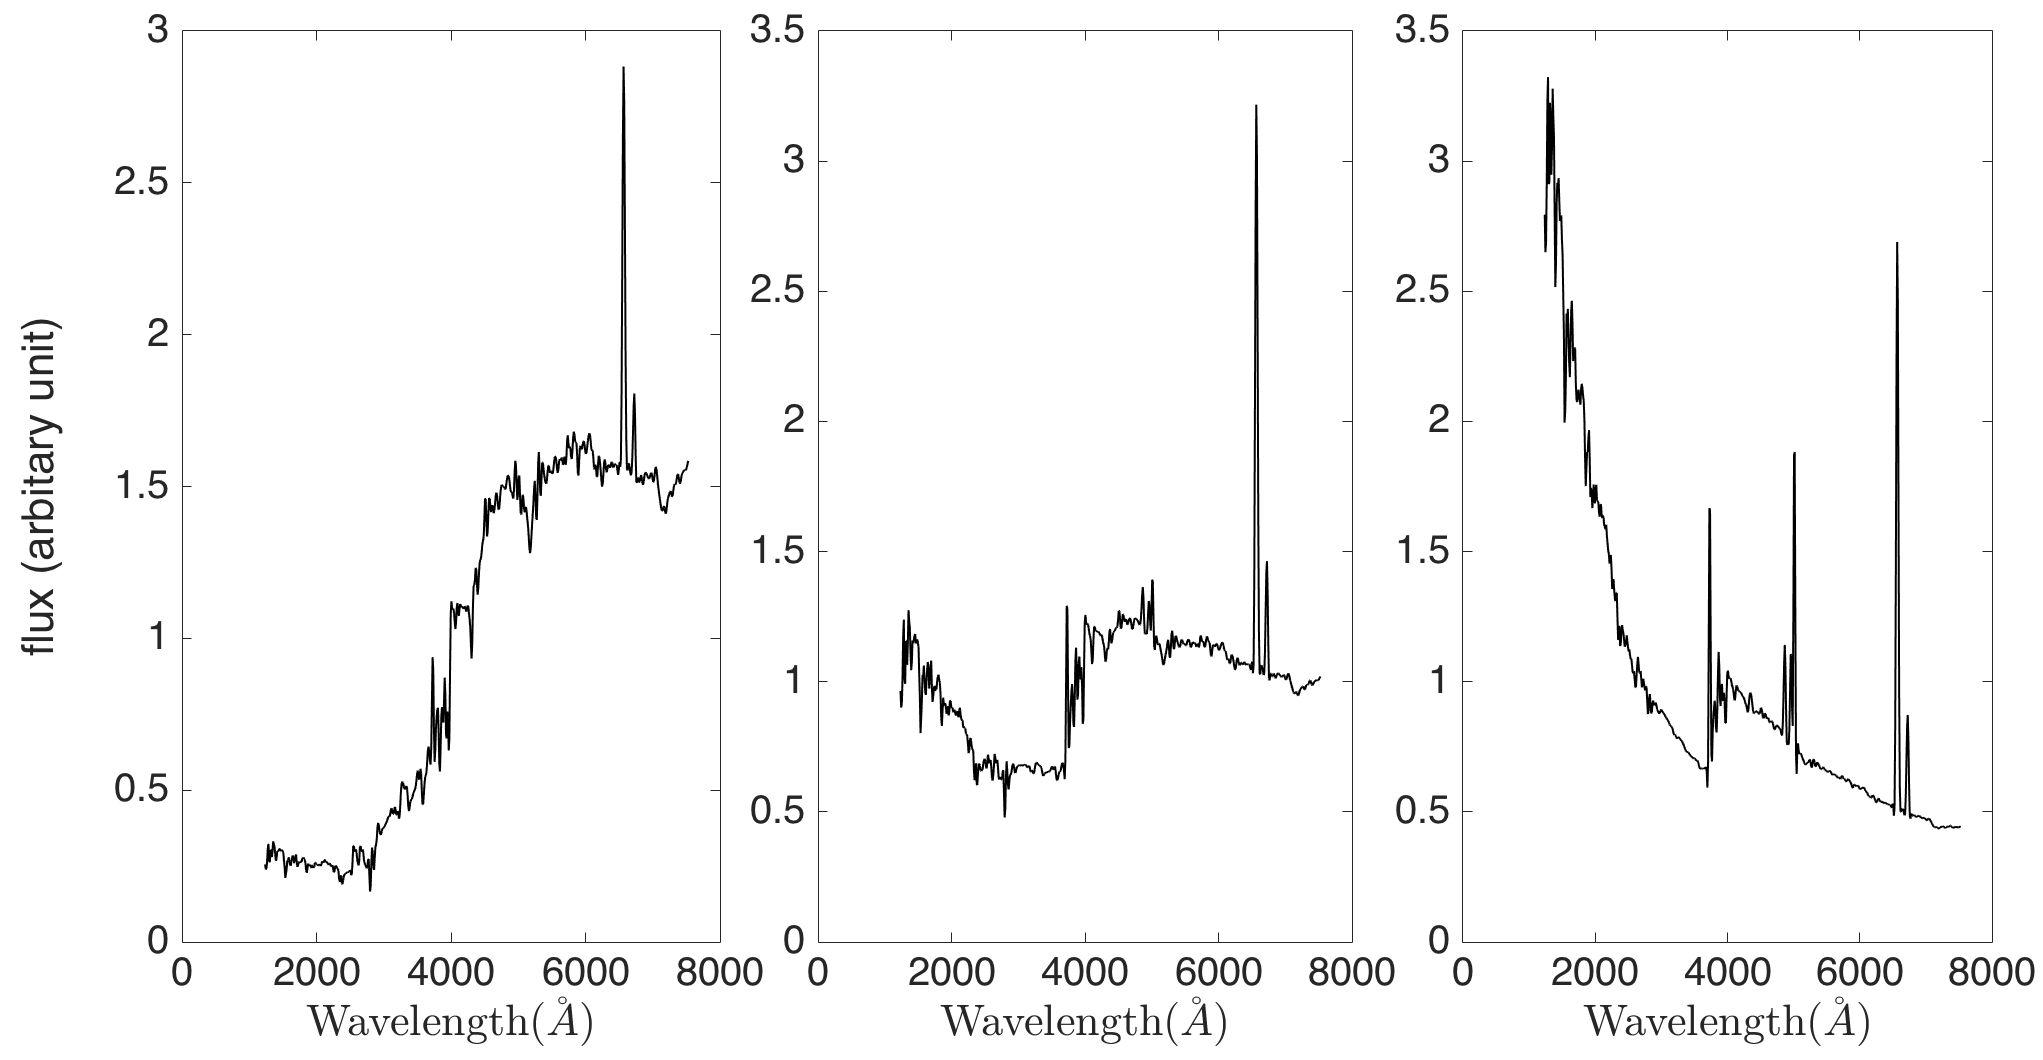
\includegraphics[width=\textwidth]{../image_paper2/1d/SED_total1by3.png}
                \end{subfigure}
                \caption[Classification of fitted galaxy SEDs from \citet{Hossein12} using the $1\times3$~networks]{Same as Fig.~\ref{fig: 1by2V}, but in this figure, we used a network with size of $1\times3$ (Fig.~\ref{fig: 1by3T}) to classify the sample galaxies.}
                \label{fig: 1by3V}
            \end{figure}       
            
            In Fig.~\ref{fig: 1by22V}, we use the $1\times22$~network to classify the sample galaxies.
            As mentioned in Section~\ref{sec: 1Dt}, in this network size we observed the first separation of the \citetalias{Kinney96} galaxies into 12 different neurons.
           As in Figs.~\ref{fig: 1by2V} and ~\ref{fig: 1by3V}, the upper panel of Fig.~\ref{fig: 1by22V} shows the number of galaxies (out of the 142) belonging to each neuron in the $1\times22$ SOM.

            \begin{figure}
                \begin{subfigure}[b]{\textwidth}
                    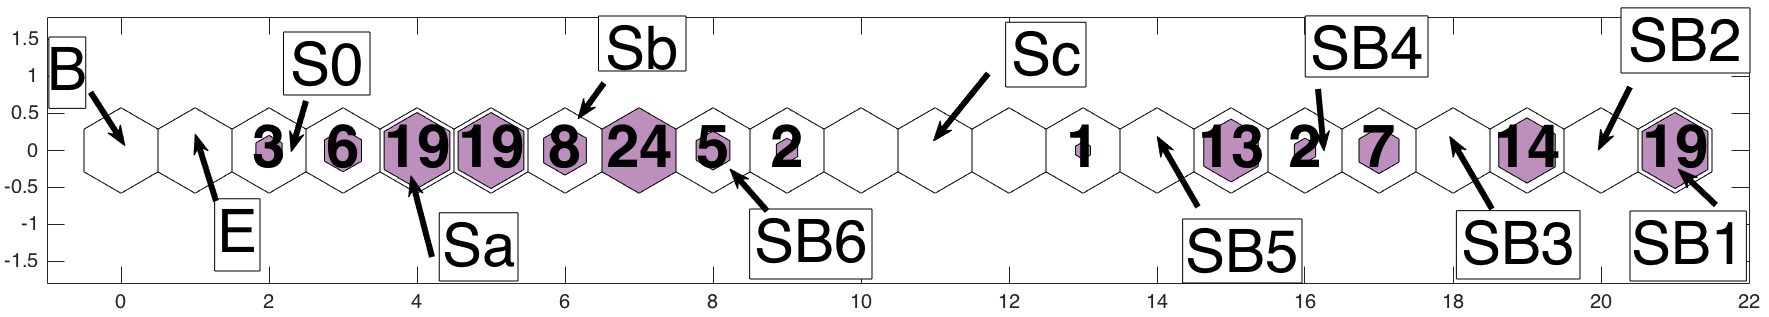
\includegraphics[width=\textwidth]{../image_paper2/1d/hit_v_1_by_22_n.png}
                    \centering
                \end{subfigure}
                \hfill
                \begin{subfigure}[b]{\textwidth}
                \centering
                     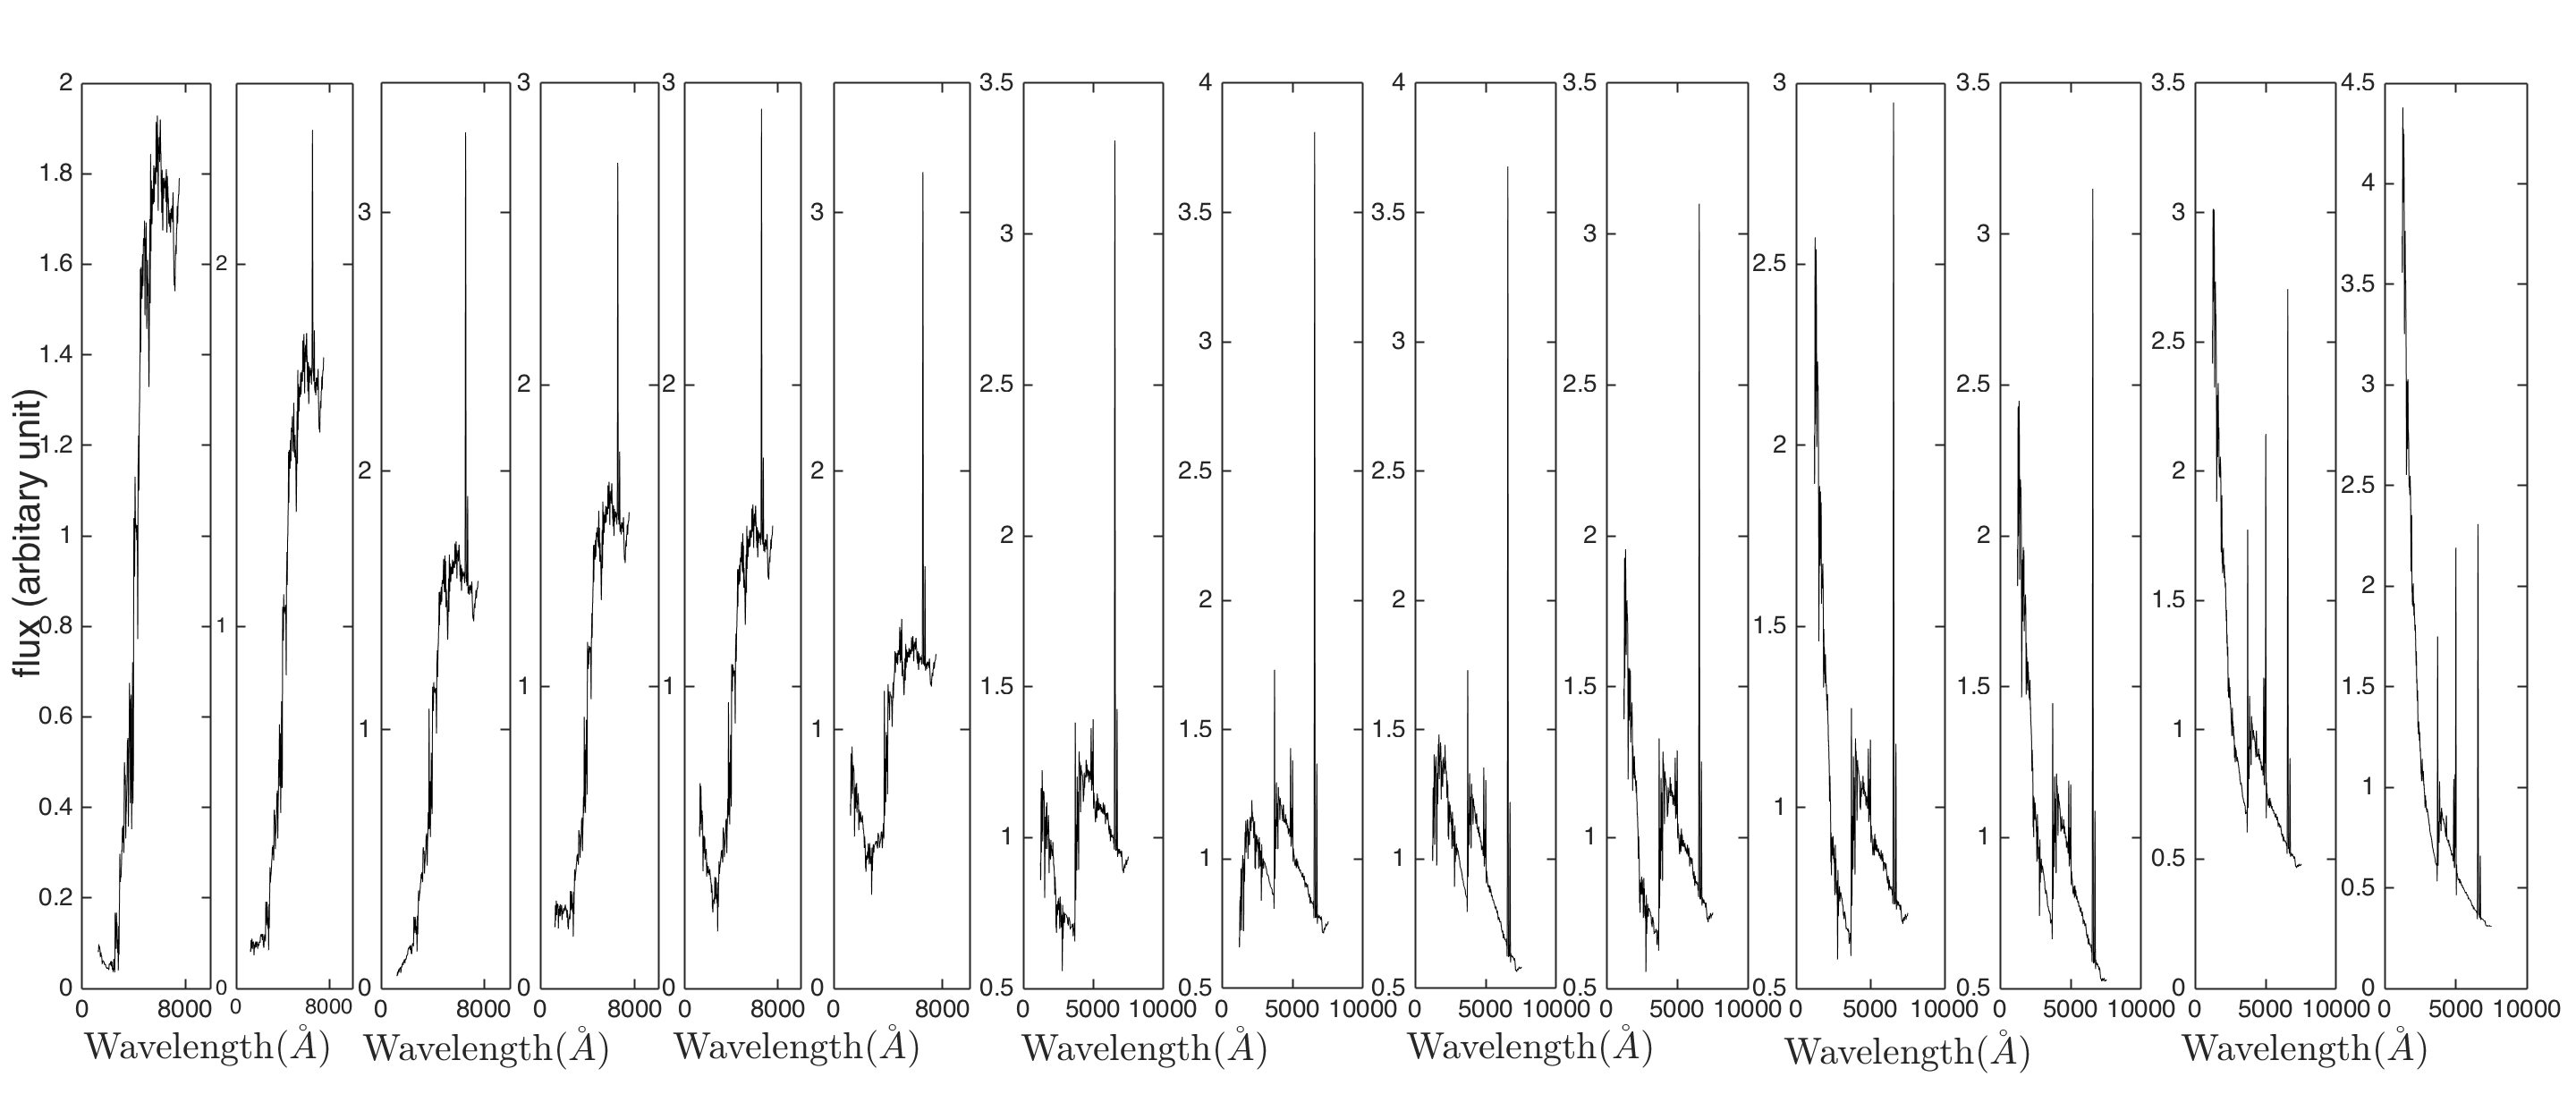
\includegraphics[width=\textwidth]{../image_paper2/1d/SED_total1by22.png}
                \end{subfigure}
                \caption[Classification of fitted galaxy SEDs from \citet{Hossein12} using the $1\times22$~networks]{Same as Fig.~\ref{fig: 1by2V}, but in this figure, we used a network with size of $1\times22$ (Fig.~\ref{fig: 1by22T}) to classify the sample galaxies. In the median spectra of each neuron, we can clearly see the changes from quiescent galaxies to the starburst ones. The 4000\AA~ break weakens from left to right and the emission line strengths increase.}
                \label{fig: 1by22V}
            \end{figure}

            The lower panels present the median spectra of the galaxies in each neuron.
            Since galaxies had more space to separate, some of the neurons are left empty.
            Thus, instead of having 22 median spectral plots in the lower part of Fig.~\ref{fig: 1by22V}, there are only 12.
            
            Comparing the upper panel of Fig.~\ref{fig: 1by22V} with the lower panel of Fig.~\ref{fig: 1by22T} shows that the occupied neurons are not necessarily the same.
            If a cluster from the \citetalias{Hossein12} sample fills the same neuron as a \citetalias{Kinney96} template, we can conclude that spectra of galaxies in the cluster are very similar to those of the template.
            Otherwise, we can conclude that the spectra of galaxies in the cluster are (dis)similar to two of the \citetalias{Kinney96} templates.
            For the latter case, the colours establish which template has greater similarity to the \citetalias{Hossein12} cluster.
            
            The first two neurons in the upper plot in Fig.~\ref{fig: 1by22V} are empty, while these neurons were occupied by galaxies B and E in the trained network.
            We therefore conclude that there are no galaxies in the \citetalias{Hossein12} sample with spectral type similar to that of type B or E.
            There are 3 galaxies in the third neuron, similar to the S0 type. 
            19 of the galaxies are jn the fifth neurons and similar to the Sa type, while the 6 galaxies in the fourth neurons have spectral type similar to both S0 and Sa galaxies.
            There are 8 Sb type galaxies and 19 galaxies with spectral types similar to both Sa and Sb type galaxies.
            The following two neurons (eighth and ninth neurons from the left) are on the edge of the quiescent and starburst galaxies.
            In the upper panel in Fig.~\ref{fig: 1by22T}, the colour between these two neurons is black, which shows that these two are very different.
            Therefore, 24 galaxies in the eighth neurons have similar spectra to Sb type galaxies, and the spectra of the 5 galaxies in the ninth neuron are similar to the SB6 galaxies.
            The far right neurons in the network belong to galaxies with spectra comparable to types SB1 and SB2.
            
            In general, 56 galaxies correspond exactly to \citetalias{Kinney96} templates and the other 86 are placed between the initial 12 suggestions.
            As \citetalias{Hossein12} mentioned, part of the reason we could not classify all the galaxies using the \citetalias{Kinney96} model is that the model was constructed from co-adding spectra of 70 galaxies.
            In this small sample, it is quite possible that the best SEDs do not match any model perfectly and the original classifications have high uncertainties.
            
            With other methods (e.g. $\chi^2$ fitting), trained neural network fitting of spectra is limited to models and the results are always reported with uncertainties.
            However, with SOM, we have the freedom to categorize galaxies in intermediate groups.
            Therefore, if the spectra of galaxies do not match completely with any of the spectra templates in Fig.~\ref{fig: k96}, they can be categorized as a spectra with similarity to two or more of the groups.

                        
        
        
        \subsubsection{Properties of the Clustered Galaxies}
        
        In order to check whether our conclusions in Section~\ref{sec: 1Dv}~are correct, in this section we test the relations between median properties of the galaxies in each neuron.
        
        \begin{figure}
            \centering
            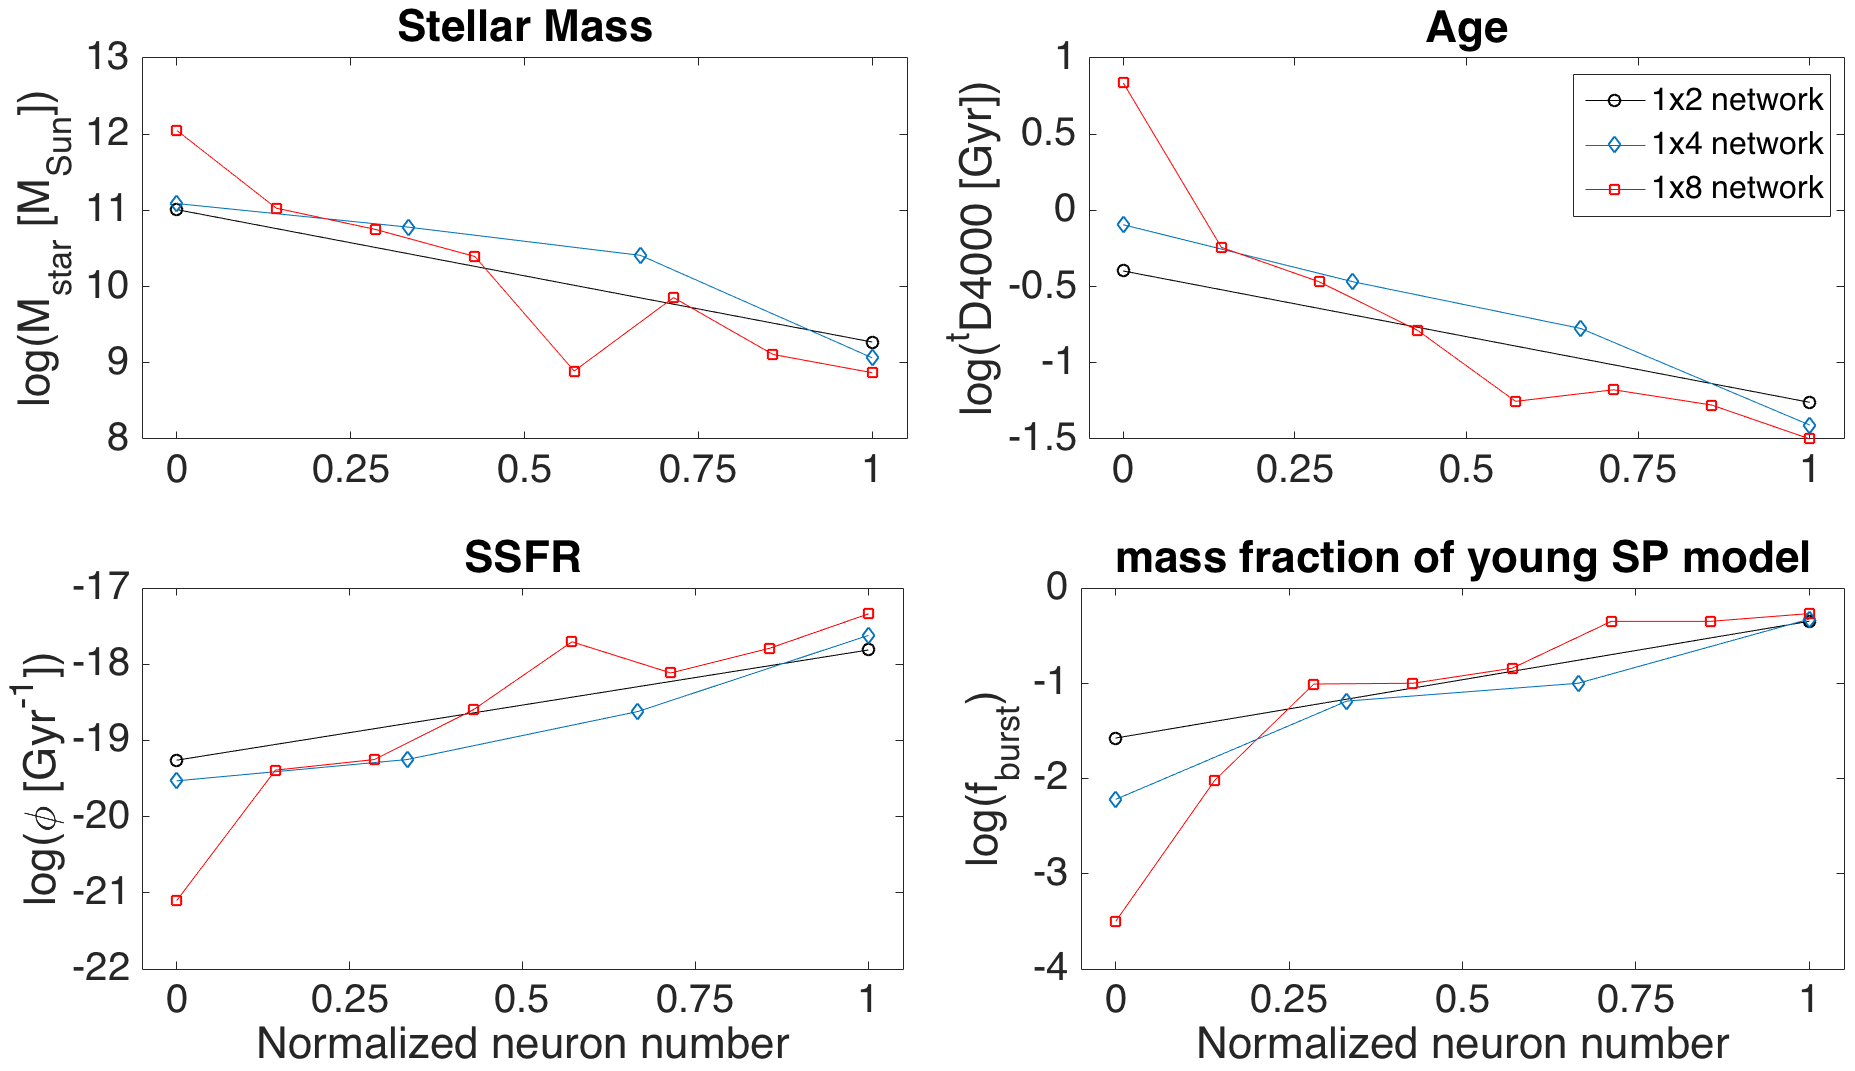
\includegraphics[width=\textwidth]{../image_paper2/1d/props5.png}
            \caption[The median of four properties of galaxies in three networks]{Comparing the median of four properties of galaxies in each node in $1\times2$ (black circles), $1\times4$ (blue diamonds), and $1\times8$ (red triangles) networks.}
            \label{fig: props}
        \end{figure}
       
        Fig.~\ref{fig: props} shows the median of stellar mass, age, specific star formation rate (sSFR; star formation rate per stellar mass), and $f_\mathrm{burst}$ of the galaxies in each neuron in the $1\times2$, $1\times4$, and $1\times8$ networks.
        In all plots, the horizontal axis is the number of the neurons divided by the size of the network.%, and vertical axis is one of the aforementioned properties.
%        
        As shown in Fig.~\ref{fig: props}, in all three networks, stellar mass and age decrease while sSFR and $f_\mathrm{burst}$ increase as the type changes from quiescent galaxies to starburst. 
       Separating galaxies based on spectral types also leads to a separation in properties that derived (via {\em CIGALE}) from the spectra, as expected since the spectra types are also based on {\em CIGALE} fitting. 
    

        {\em CIGALE} has various models to derive the properties of galaxies.
        Through these models, some of the properties are already known to be correlated with each other, e.g., stellar mass and star formation rate.
        \citetalias{Noll09} studied other relations between properties with no direct correlation in the models in a sample of SINGS galaxies.
        They found a tight correlation between sSFR and t$_{\rm {D4000}}$, which suggests that younger stellar population correlates with higher SFR.
        They also found correlations between stellar mass and SFR, and stellar mass and t$_{\rm {D4000}}$.
        Since in the {\em CIGALE} code, stellar mass is a free parameter, \citetalias{Noll09} argued that any stellar-mass-related correlation must be astrophysically meaningful. 
        They also studied relations between the attenuation at 1500 \AA~(A$_{\rm {FUV}}$) and sSFR, age, and stellar mass and did not find any correlation.
        \citetalias{Hossein12} replicated the upper plots in Fig.~\ref{fig: props_vs_props}, and found a tighter correlation than \citetalias{Noll09} results. 
        
        \begin{figure}
        \begin{subfigure}[b]{0.3\textwidth}
            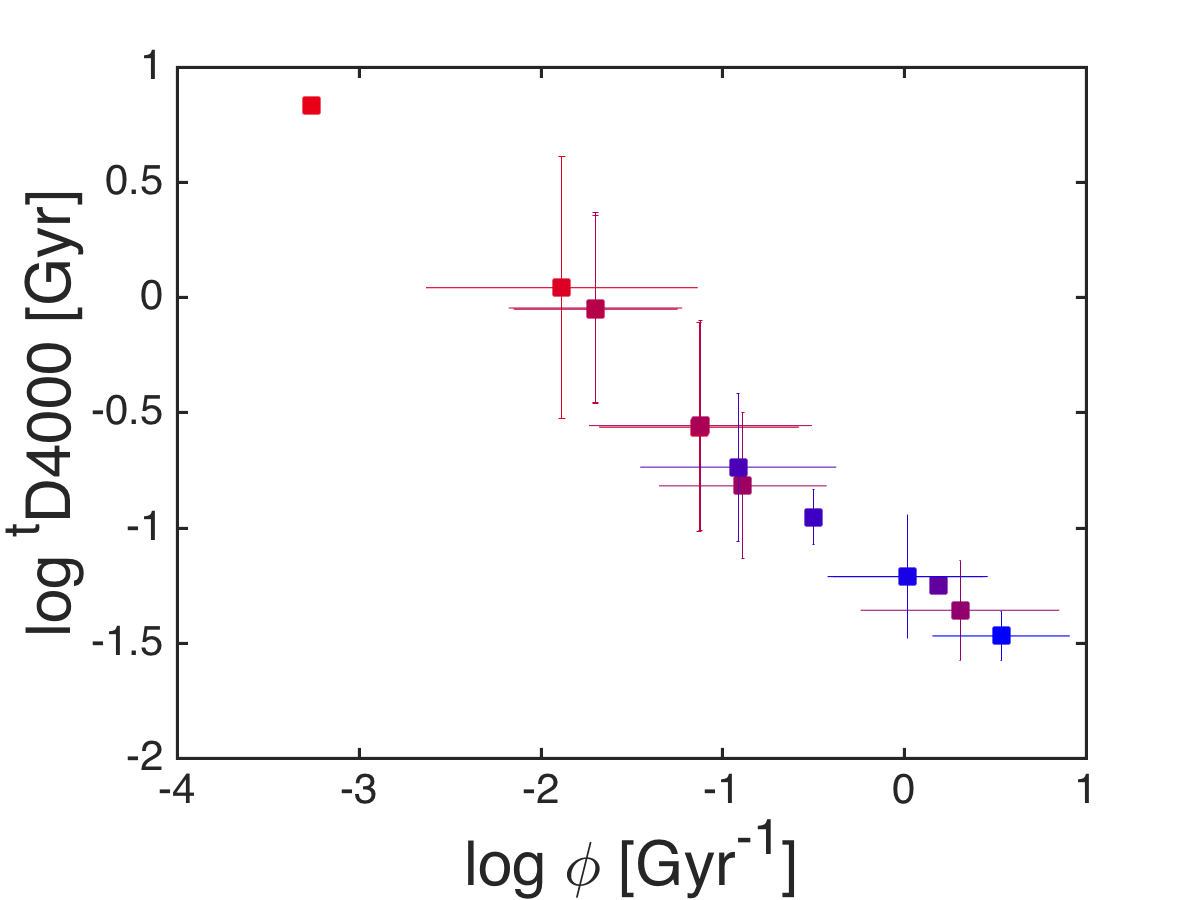
\includegraphics[width=\textwidth]{../image_paper2/1d/f1.png}
        \end{subfigure}
        \hfill
        \begin{subfigure}[b]{0.3\textwidth}
            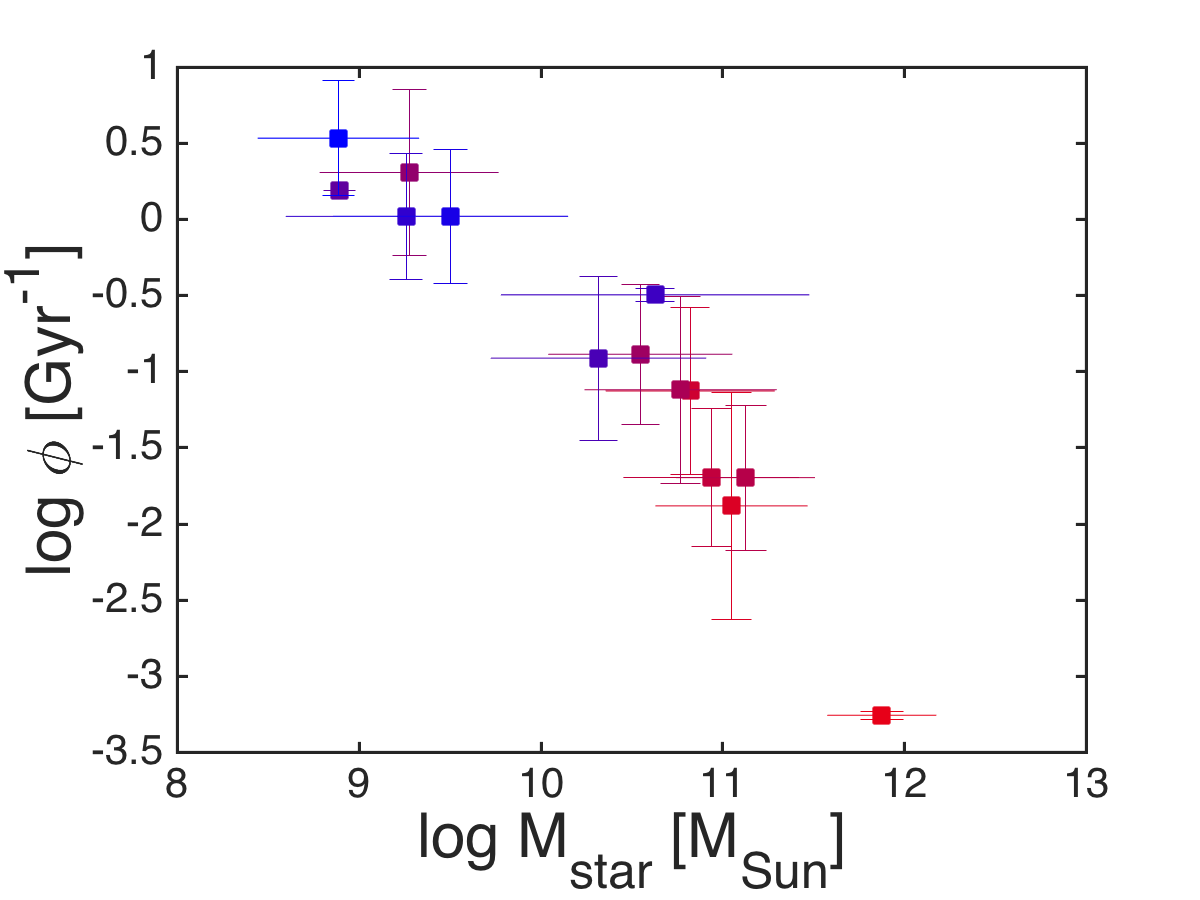
\includegraphics[width=\textwidth]{../image_paper2/1d/f2.png}
        \end{subfigure}
        \hfill
        \begin{subfigure}[b]{0.3\textwidth}
            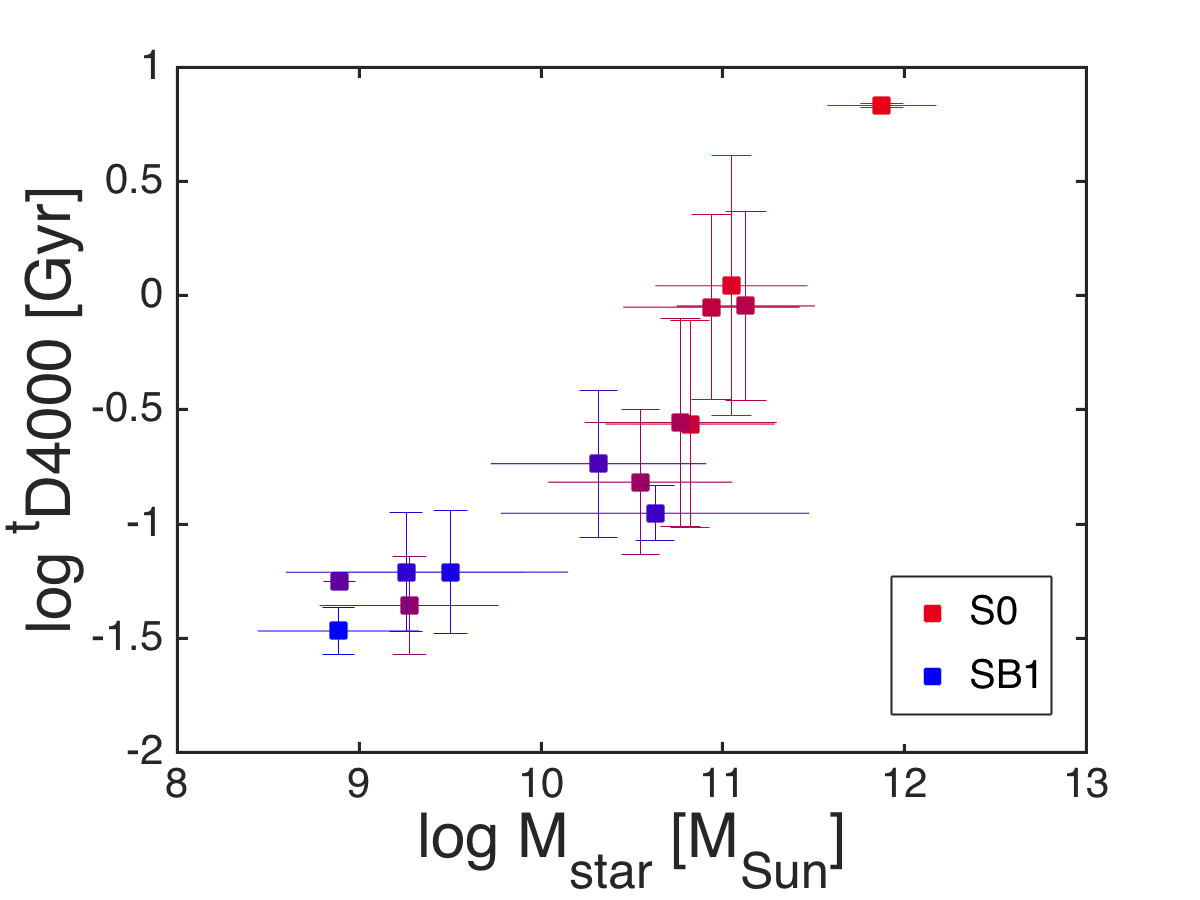
\includegraphics[width=\textwidth]{../image_paper2/1d/f3.png}
        \end{subfigure}
        \hfill
        \begin{subfigure}[b]{0.3\textwidth}
            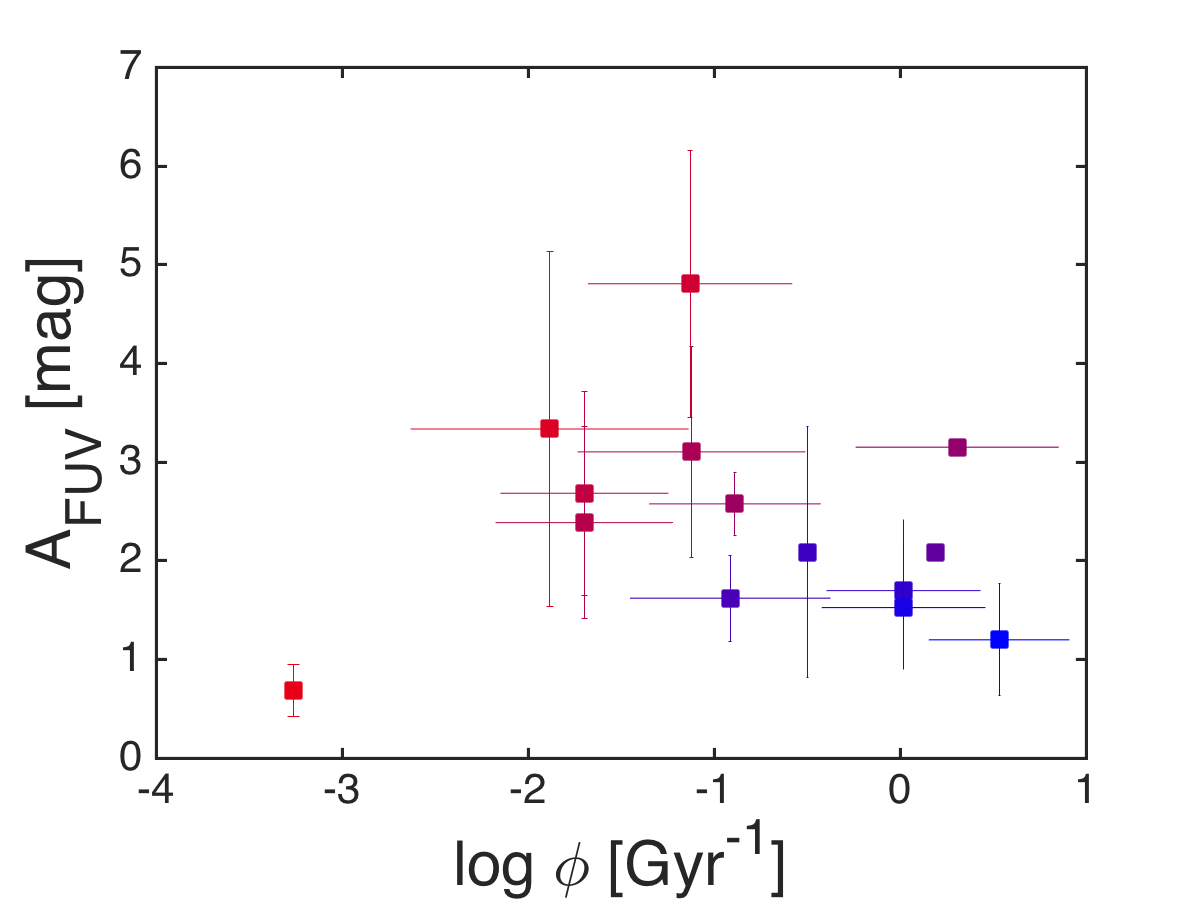
\includegraphics[width=\textwidth]{../image_paper2/1d/f4.png}
        \end{subfigure}
        \hfill
        \begin{subfigure}[b]{0.3\textwidth}
            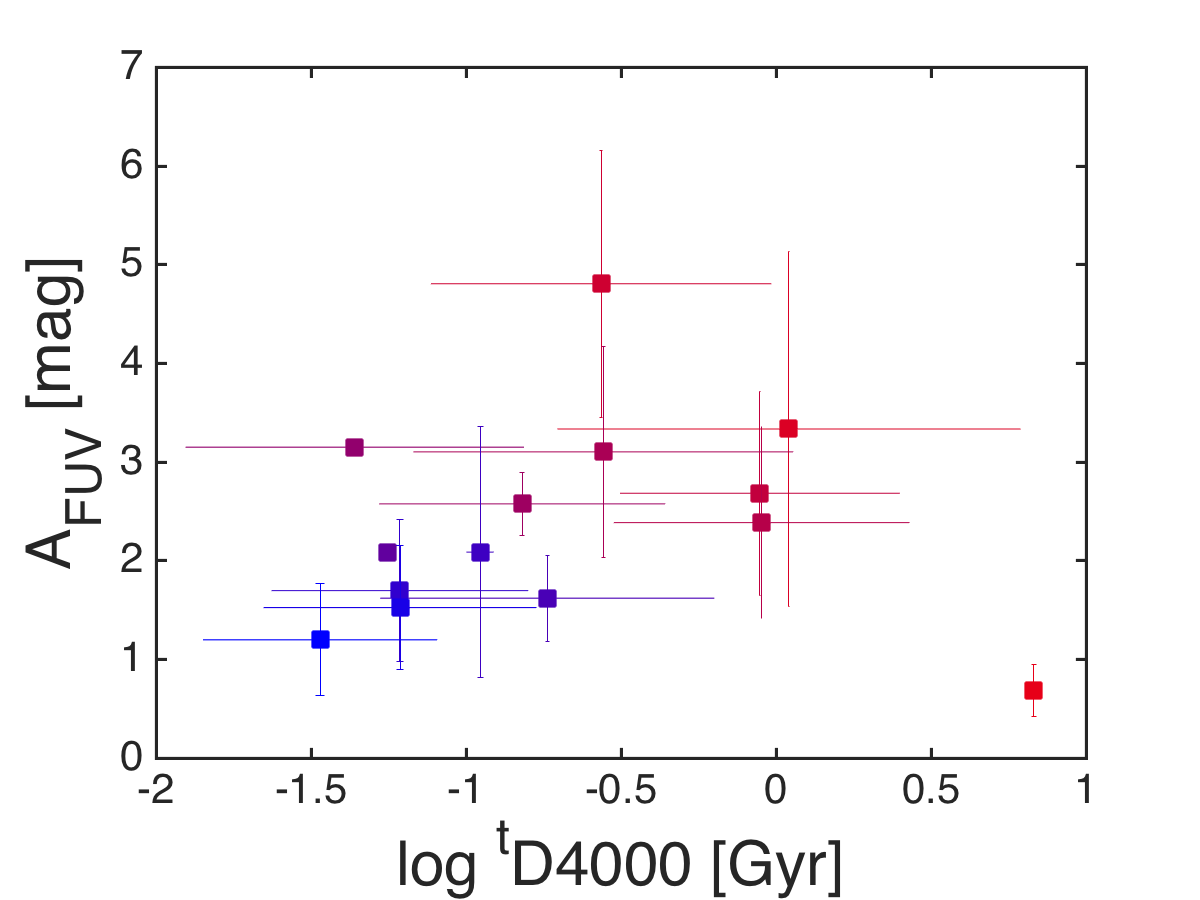
\includegraphics[width=\textwidth]{../image_paper2/1d/f5.png}
        \end{subfigure}
       \hfill
        \begin{subfigure}[b]{0.3\textwidth}
            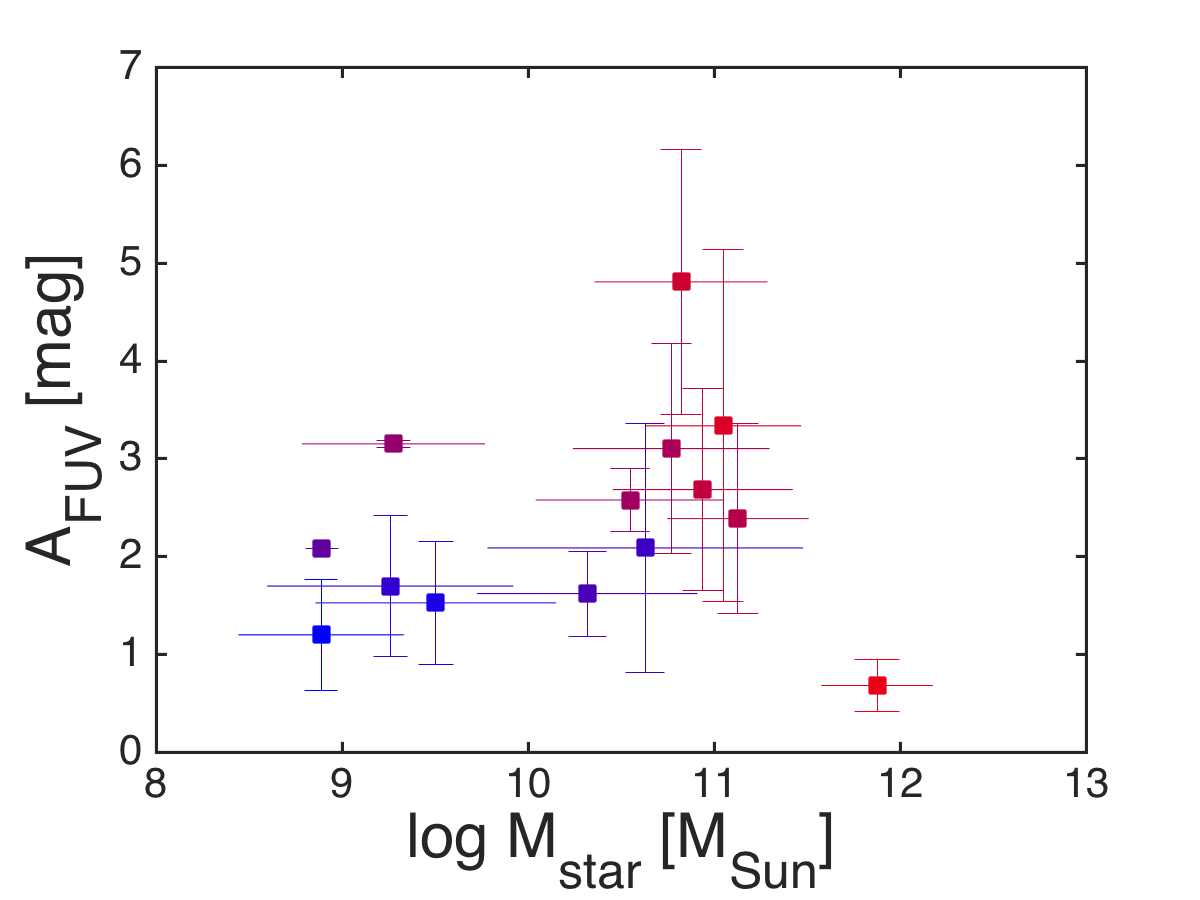
\includegraphics[width=\textwidth]{../image_paper2/1d/f6.png}
        \end{subfigure}
        \caption[Relations between properties of the clustered galaxies]{From top to bottom: Correlation between age (t$_{\rm {D4000}}$) and sSFR ($\phi$), sSFR and stellar mass, age (t$_{\rm {D4000}}$) and stellar mass, and A$_{\rm {FUV}}$ with sSFR, age (t$_{\rm {D4000}}$) and stellar mass. Points show the median values of these properties of galaxies in $1\times22$ network and error bars are the standard deviation of the median values. colours shows the type of the galaxies in the new classification. The most pure red colour shows E type galaxies and the most blue one indicates the SB1 galaxies. The other colours depend on how much they are close to red or blue show that the galaxies are quiescent or starburst.}
        \label{fig: props_vs_props}
    \end{figure}
        
        In order to compare our classifications with previous work, we produced similar plots to the ones in both \citetalias{Noll09} and \citetalias{Hossein12} (Fig.~\ref{fig: props_vs_props}).
        In Fig.~\ref{fig: props_vs_props}, the data points are median values of the properties of the galaxies in each neuron in Fig.~\ref{fig: 1by22V}, and error bars show the standard deviation of those properties.
        The colours show the galaxy types, where B type galaxies are shown with red and SB1 types are shown with blue.
        The redder the colour, the more similarity with quiescent galaxies, while the purple to blue colours show more similarity to starburst galaxies.
        Since in this method we allow galaxies to occupy classes in between the original \citetalias{Kinney96} templates, we have more than 12 colours in Fig.~\ref{fig: props_vs_props}.
        The purple point in the middle of the blue points in Fig.~\ref{fig: props_vs_props} corresponds to galaxies with spectra similar to type Sc: the shape of their spectra indicates that they are old galaxies with high sSFR.
        
        The upper panels in Fig.~\ref{fig: props_vs_props} show the same relations as \citetalias{Noll09} and \citetalias{Hossein12}, but with tighter correlation than those two, in all three plots.
        As mentioned in both \citetalias{Noll09} and \citetalias{Hossein12}, galaxies with smaller mass tend to be younger and more active.
        Fig.~\ref{fig: props} shows similar results: younger and more active galaxies have less stellar mass and more f$_{\rm {burst}}$.
        From older to younger galaxies, the colour of the points changes from red to blue, which shows a good correlation with their spectral type.
        %for more details discussion on these correlations, we encourage readers to read \citetalias{Noll09} and \citetalias{Hossein12}.
        
        \citetalias{Noll09} studied a correlation between A$_{\rm {FUV}}$ and other properties of galaxies and showed that the attenuation has no dependence on the specific star formation or age.
        In contrast to \citetalias{Noll09}, we find a correlation between A$_{\rm {FUV}}$ and these two parameters, shown in the lower panels of Fig.~\ref{fig: props_vs_props}.
        The general trend of the correlation between A$_{\rm {FUV}}$ and sSFR in Fig.~\ref{fig: props_vs_props} is similar to the trend found by \cite{Dale07}.
        They used IR luminosity to UV luminosity ratio (L$_{IR}$/L$_{FUV}$) as a measure of A$_{\rm {FUV}}$ and compared it with sSFR for all 75 galaxies in the SINGS survey.
        They found that for quiescent galaxies (E, S0 and S0/a ), L$_{IR}$/L$_{FUV}$ (or A$_{\rm {FUV}}$ ) correlates with sSFR, and for spiral galaxies, there is an anticorrelation between L$_{IR}$/L$_{FUV}$ and sSFR.
       Since our sample has no E-type galaxies, we cannot confidently show the same correlation between A$_{\rm {FUV}}$ and sSFR. 
        However, it is clear in Fig.~\ref{fig: props_vs_props} that A$_{\rm {FUV}}$ increases with increasing sSFR in the S0 and Sa types.
        The correlation in the other types of galaxies is very similar to the one shown by \cite{Dale07}.
        Both \cite{Dale07} and \citetalias{Noll09} argued that these apparent trends can be a result of the dependence of star formation history on L$_{IR}$/L$_{FUV}$.
        Whether this dependence is real or not, our results here show that using self-organizing maps can separate spectra of galaxies in such a way that the characteristics of each of these groups are in agreement with the general picture of the galaxy evolution.
      
    \subsection{Two-Dimensional Self-Organizing Maps}
    \label{sec: 2D}
    The one-dimensional networks are great tools to categorize the spectral types of galaxies and monitor the changes of properties of galaxies with category.
    However, each neuron in these networks is limited to be connected to one other neuron in each direction.
    In a 2D network, each neuron can have more than two immediate neighbours, providing a more complete pictures of relations between each spectral type.
    As described in Section~\ref{sec: method_somz}, one of the main advantages of the SOM is that when the weight of one neuron is adjusted after finding the best matching unit, the weight of the whole map will be changed.
    This quality of the SOMs provides a unique opportunity to analyse 2D networks using two approaches. 
    At first, as in the 1D SOMs, we assumed that all the galaxies must have spectra similar to any of the 12 templates in Fig.~\ref{fig: k96}.
    In this case, we can categorize spectra of other galaxies based on those 12 types.
    In the second approach, we trained networks with the assumption that there might be completely different types of galaxies not encountered before.
    This approach can be used to trace and recognize the outliers, which could include galaxy types that are not presented in the \citetalias{Kinney96} templates.
    To execute the second approach, we used the {\textsc selforgmap} library in the {\textsc matlab}.
    Unlike the {\textsc newsom} library which the ordering step neighbourhood distance is set by default (although in an SOM it should be a free parameters), in the {\textsc selforgmap} we can change this value.
    Using the {\textsc selforgmap} code, based on the size of a map and the ordering step neighbourhood distance, we can arrange that the data spread all over the SOM or sit close together, allowing room for outliers.

    To get the best result from both methods, we should have SOMs with ``enough"  neurons to give any new types of galaxies a chance to find their places in the map.
    ``Enough neurons" is a vague statement, but as mentioned in the Section~\ref{sec: method_somz} the size of SOMs is arbitrary and depends on the size of the input data and the kind of information needed from the SOMs.
    Since the training dataset (the \citetalias{Kinney96} templates) has 12 members, we assumed a SOM with size of $8\times8$~would be a good start.
    We then increased the size of the SOM to find the highest size suitable for the training sample.
    We noticed that very few changes occurred after the SOMs were grown to a size greater than $12\times12$, so we used this as the maximum size.
    
    \begin{figure}
        \begin{subfigure}[b]{0.45\textwidth}
            \centering
            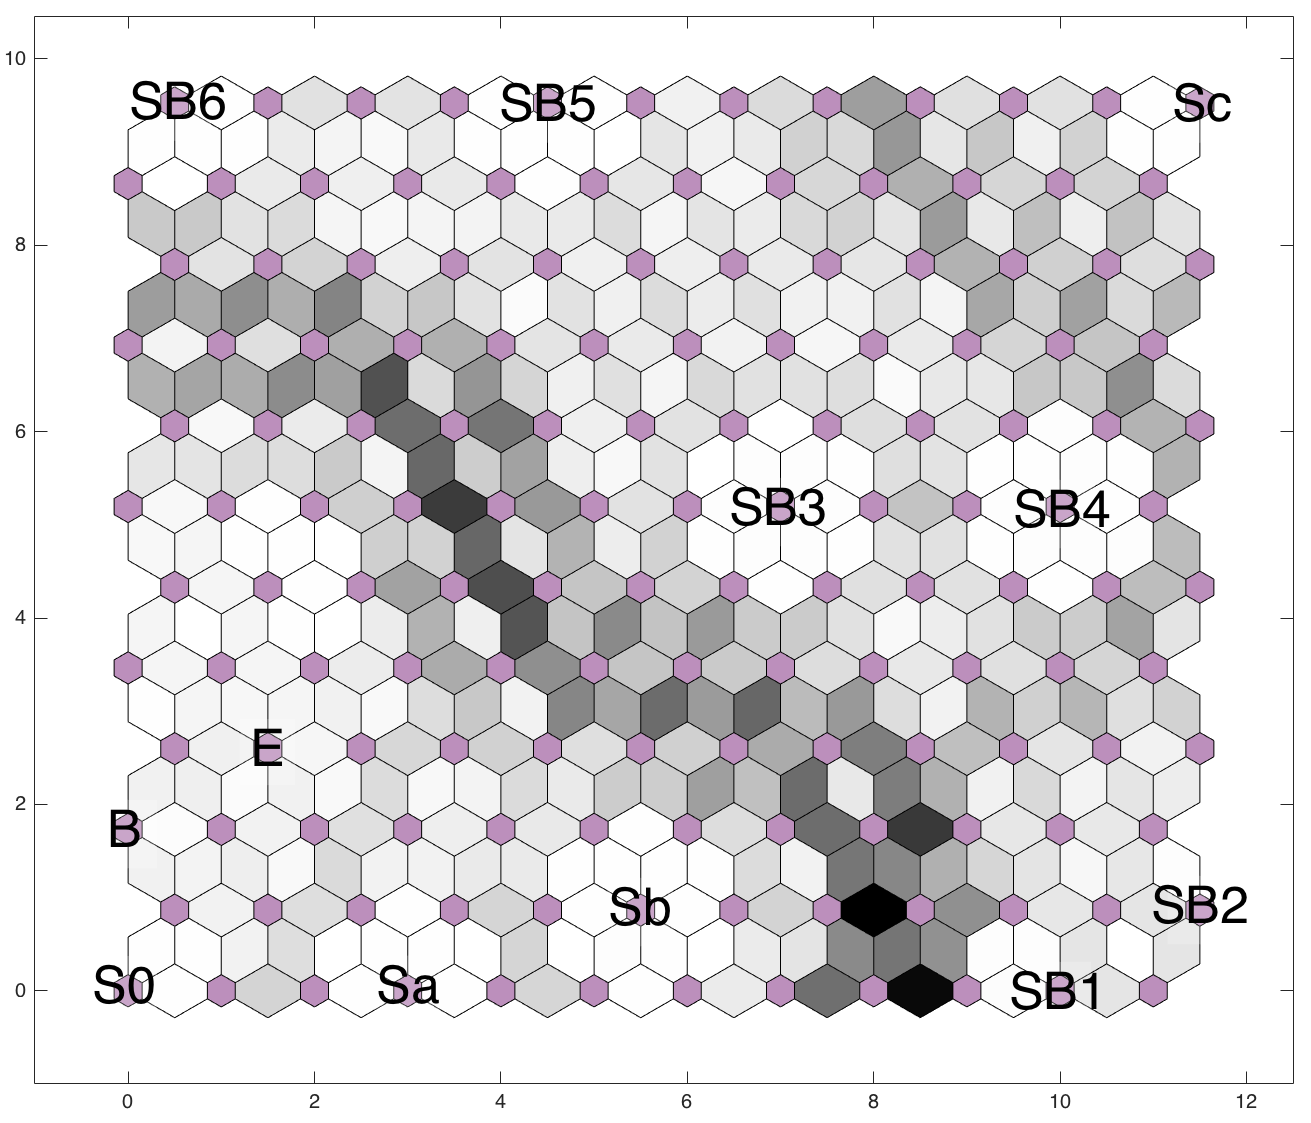
\includegraphics[width=\textwidth]{../image_paper2/2d/dist_12_by_12.png}
        \end{subfigure}
        \hfill
        \begin{subfigure}[b]{0.45\textwidth}
            \centering
            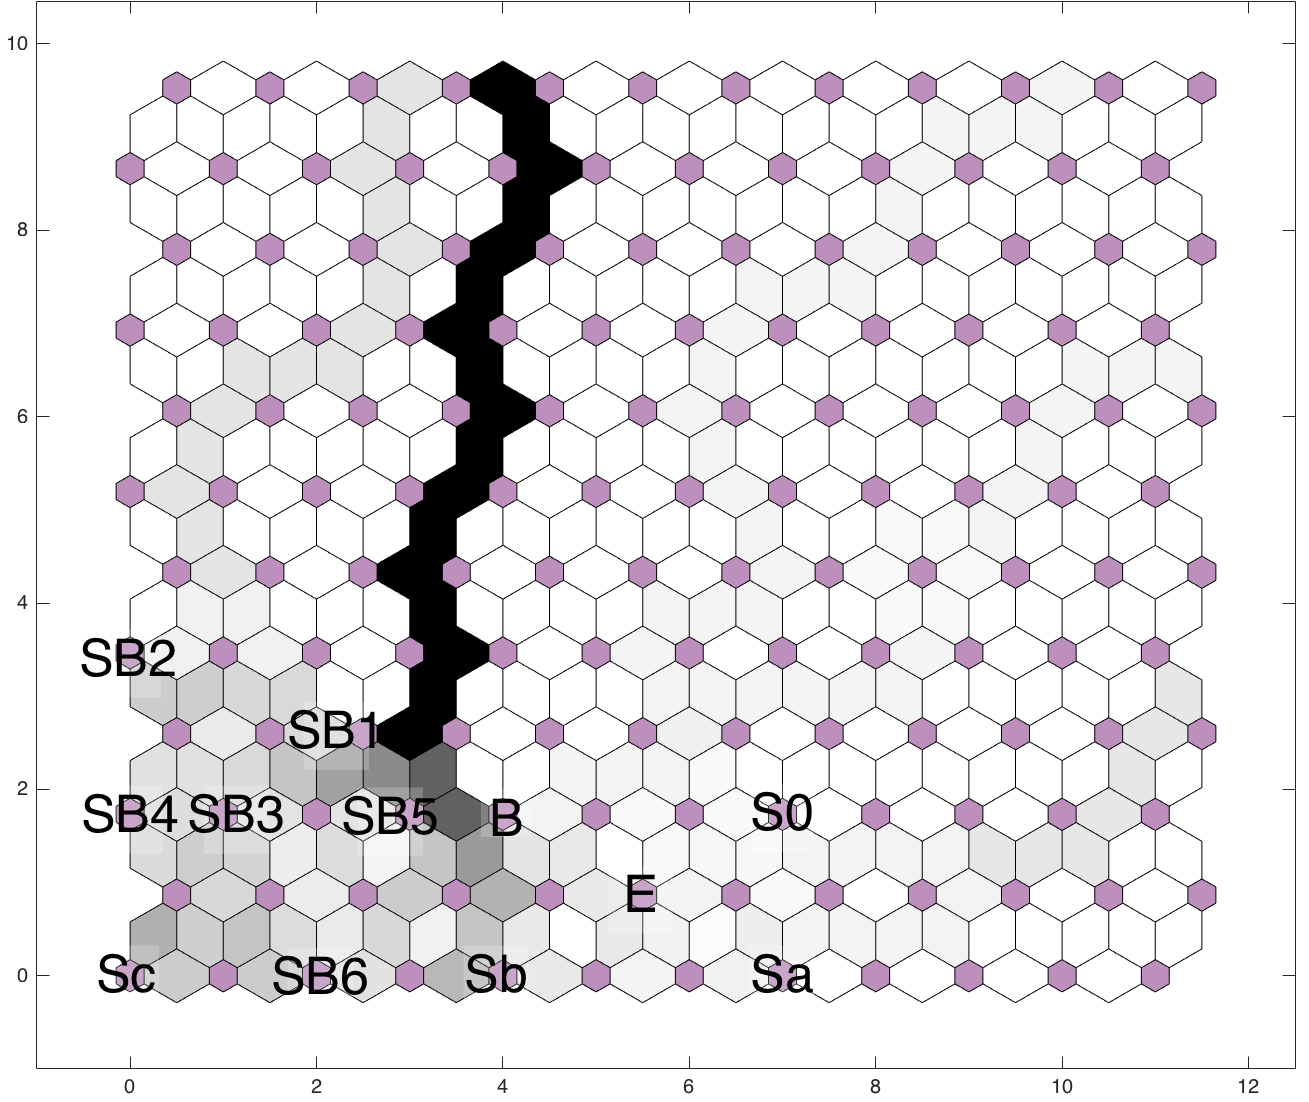
\includegraphics[width=\textwidth]{../image_paper2/2d/dist_12_by_self_org_res12.png}
        \end{subfigure}
        \hfill
        \begin{subfigure}[b]{0.45\textwidth}
            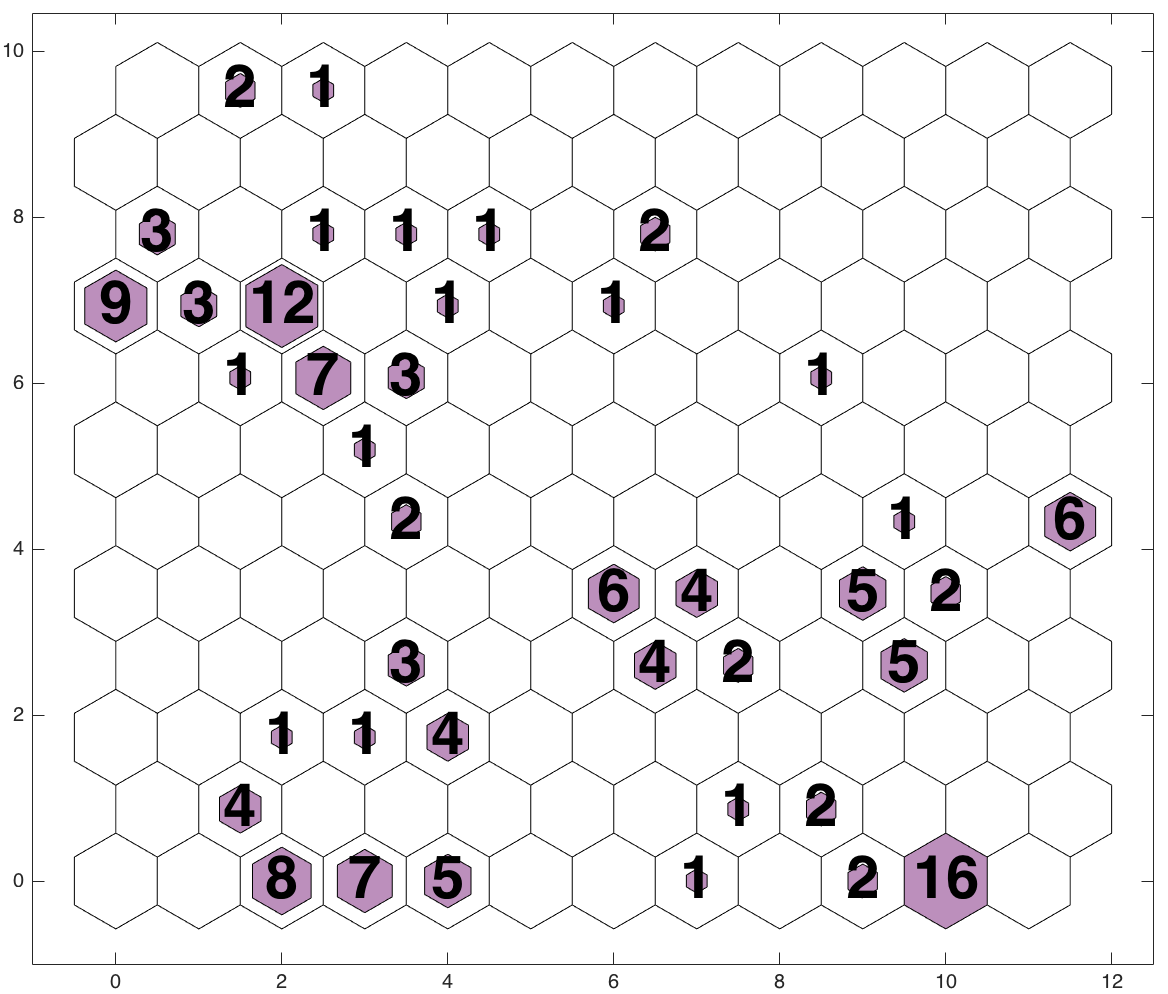
\includegraphics[width=\textwidth]{../image_paper2/2d/hit_v_12_by_12.png}
        \end{subfigure}
        \hfill
        \begin{subfigure}[b]{0.45\textwidth}
            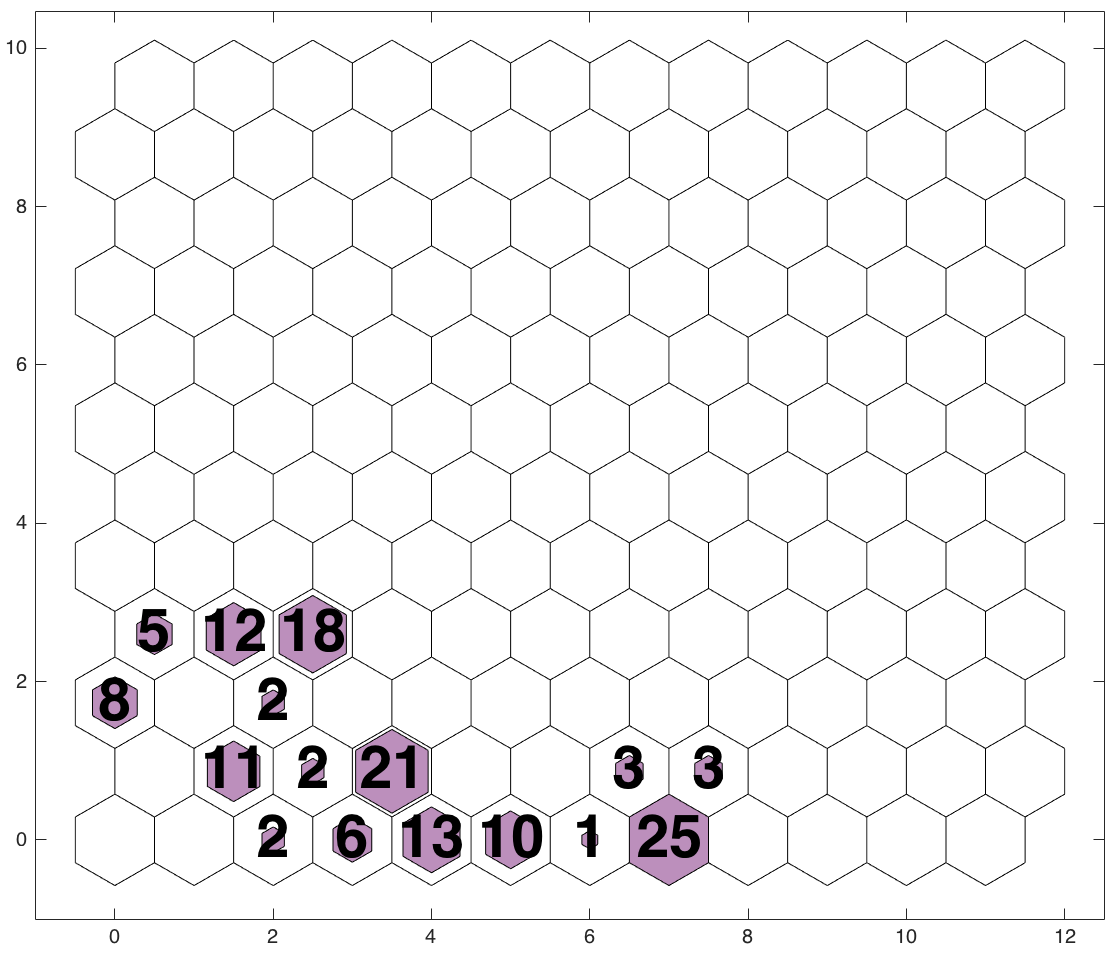
\includegraphics[width=\textwidth]{../image_paper2/2d/hit_v_12_by_self_org_res12.png}
        \end{subfigure}
        \caption[$12\times12$ two-dimensional self-organizing map results]{$12\times12$~2D SOM results. Upper panel: SOMs trained using the \citet{Kinney96} templates. For training 2D SOMs two different approaches were considered: either only 12 types of galaxies exist (left) or not (right). Lower panel: classifying the galaxies from \citetalias{Hossein12}, using the trained networks shown in the upper panels. From the lower right panel, we can see that there are no outliers in the galaxies from \citetalias{Hossein12}, and we can use the map in the lower left panel as a final clustering result for the \citetalias{Hossein12} galaxies.}
        \label{fig: 12by12}
    \end{figure}
    
    The upper left panel in Fig.~\ref{fig: 12by12} shows the SOM results from the first approach. 
    Since we considered that spectra of all galaxies can be categorized using the \citetalias{Kinney96} templates, the galaxies were placed all over the map.
    Using this network to categorize any set of spectra forced the spectra to be either in the same neurons as the \citetalias{Kinney96} templates or in the neurons between them.
    In the map shown in the upper right panel in Fig.~\ref{fig: 12by12}, the \citetalias{Kinney96} templates are in a small region. This provides enough freedom for the spectra of galaxies to be placed everywhere in the map, even far away from the templates.
    
    
    In the upper left part of the map in Fig.~\ref{fig: 12by12}, although galaxies have more ways to be separated, they were separated in two main groups.
    There is a distinguishable strip of grey, dark grey and in some cases black colour in the map:
    this strip separates quiescent galaxies from starburst ones.
    The lower map shows that 5 of the neurons on the left side of the strip are full. 
    These five neurons are the same as the ones on the left hand side of Fig.~\ref{fig: 1by2T} (quiescent galaxies),
    the only difference being that in this map they have more space to be separated from each other.
    When we use this network to categorize the spectra of galaxies, any galaxy placed on the left hand side of the strip is a quiescent galaxy and any one placed on the right side of the strip is a starburst one.
    The decision about what sub-type of quiescent or starburst galaxy is based upon its relative position to each type in the SOM.
    
    As in the other map, in the upper right panel of Fig.~\ref{fig: 12by12}, galaxies are generally divided into two main groups.
    The border between the quiescent galaxies and the starburst ones is the black strips in the middle of the map,  ending with the bright grey colour at the bottom of the map in the fifth neuron.
    In this network, neurons in the right side of the strip represent the quiescent galaxies and the neurons in the left side represent the starburst ones. 
    When categorizing a new set of spectral types, if the new spectra are similar to the \citetalias{Kinney96} template all of them will be placed in the bottom of the map, but if there are different type of galaxies, they would sit in any other neurons in the map.
    In large datasets, one can easily use this network to figure out whether there is any of new type of spectra (or any outliers) in the datasets. 
    Since the networks are already available, this procedure should be quick and easy for big datasets.
    
    We used both 2D networks to categorize the \citetalias{Hossein12} galaxies and the results are shown in the lower panels of Fig.~\ref{fig: 12by12}.
    In the lower right map in Fig.~\ref{fig: 12by12}, all galaxies are placed in the bottom part of the map and we can conclude that in the \citetalias{Hossein12} sample there are no outliers or spectra with very different from the \citetalias{Kinney96} templates.
    The lower left map of Fig.~\ref{fig: 12by12} shows the \citetalias{Hossein12} galaxies categorized based on the network in the upper left of Fig.~\ref{fig: 12by12}. 
    Comparing this categorization with the 1D one from Fig.~\ref{fig: 1by22V}, we can see that only 23 galaxies correspond exactly to \citetalias{Kinney96} types.
    Using 2D maps results in categorizing galaxies into more intermediate type than in 1D maps.
    In both lower maps in Fig.~\ref{fig: 12by12}, most galaxies are in the quiescent side of the SOM, which was predictable from the results in Sec.\ref{sec: 1Dv}. This does not imply that in general there are more quiescent galaxies at higher red-shifts but rather is a selection effect from the fact that those galaxies had more reliable redshift estimates.
    
    Although for ease of presentation this paper first discusses 1D networks and continues to 2D networks, we suggest that users of SOMs for galaxy spectral classification should use 2D networks first. These can be used as a first step with networks similar to the upper left map in Fig.~\ref{fig: 12by12} to identify outliers in the sample.


%----------------------------------------------------------------------------------------
%----------------------------------------------------------------------------------------
%----------------------------------------------------------------------------------------
%Summery
%----------------------------------------------------------------------------------------
%----------------------------------------------------------------------------------------
%----------------------------------------------------------------------------------------
\section{Summary and Future Applications}
\label{sec: summary_SOMZ}

Self-organizing maps can be used to classify celestial objects (e.g. stars, quasars, spectra of galaxies, light curves, etc.)
Galaxy spectra can be classified in various networks with different sizes/dimensions based on the information needed from the data. 
If a broad and general classification is required, networks can have one dimension with a few neurons.
If one needs more detailed classifications, a higher number of neurons should be used.
Since self-organizing maps do not include the uncertainty of input parameters, sometimes too much attention to detail can cause problems in classifications. 
%Some small differences could easily be the result of atmosphere fluctuation or other instrumental or observational problems. 
When using the SOM method, one should consider whether small differences between objects are physically meaningful when separating two groups from each other.

We used SOMs to classify the template spectra of \citetalias{Kinney96}, made from galaxies with known morphological type, and created networks with different uses.
By varying the size of the networks, we found the relative similarity between the \citetalias{Kinney96} template classes.
A one-dimensional network with 22 neurons was needed in order to
separate all 12 \citetalias{Kinney96} spectra; we concluded that \citetalias{Kinney96} types B and E, and types SB1 and SB2, are very similar to each other.
We also showed that networks generated with the SOM method can be used to easily identify new types of spectra in large surveys.

A sample of 142 high red-shift galaxies from \citetalias{Hossein12} was used to test the trained networks.
%One of the main criteria to choose a test sample is that the test sample must have fluxes in exactly the same wavelengths of the training sample.
The test results showed that using SOMs can allow identification of galaxies with spectra similar to two or more morphological types.% but not exactly the same as one of them.
The freedom of having in-between types is one of the main differences between supervised and unsupervised artificial neural networks.
\citetalias{Hossein12} used a supervised training method to train networks with \citetalias{Kinney96} spectral templates and classify the same sample of 142 galaxy spectra;
however, they could not classify 37 out of 142 spectra.
The unsupervised method used in this project was able to classify all 142 spectra in the sample
as belonging to one of the morphological types introduced by \citetalias{Kinney96} or a class in between those types.

The properties of the galaxies in the test sample using the new
classification were found to more tightly correlate in mean values of age, specific star formation rate, stellar mass, and far-UV extinction than in previous studies. 
The properties of the galaxies in each group are in good agreement with their morphological types.

Two-dimensional networks can be used to find the relations of the neurons and classifications in more details.
The sample galaxies have more freedom to be categorized, and only 23 of them occupies exactly the same neurons as \citetalias{Kinney96} template spectra (in one-dimensional networks this number was 56).
Additionally, by using two-dimensional networks we showed that we do not have nay outlier in the sample galaxies.


\addcontentsline{toc}{section}{Bibliography}
\bibliographystyle{apj.bst}
\bibliography{ref_paper2.bib}